\documentclass{jfm}

\usepackage{graphicx}
%\usepackage{epstopdf,epsfig}
\usepackage{newtxtext}
\usepackage{newtxmath}
\usepackage{natbib}
\usepackage{hyperref}
\usepackage{subfigure}
\usepackage{overpic}
%\usepackage{cite}
\usepackage{tikz}
\hypersetup{
	colorlinks = true,
	urlcolor   = blue,
	citecolor  = black,
}
\newtheorem{lemma}{Lemma}
\newtheorem{corollary}{Corollary}
\newcommand{\RomanNumeralCaps}[1]

\graphicspath{{./Figures}}

% {\MakeUppercase{\romannumeral #1}}

%% new commands for partial derivatives
\newcommand{\pddt}[1]{\dfrac{\partial #1}{\partial t}} %partial d/dt 
\newcommand{\pddr}[1]{\dfrac{\partial #1}{\partial r}} %partial d/dr	
\newcommand{\pddx}[1]{\dfrac{\partial #1}{\partial x}} %partial d\dx
\newcommand{\pddy}[1]{\dfrac{\partial #1}{\partial y}} %partial d\dy
\newcommand{\pddz}[1]{\dfrac{\partial #1}{\partial z}} %partial d\dz
\newcommand{\pddZ}[1]{\dfrac{\partial #1}{\partial Z}} %partial d\dZ
\newcommand{\pdbyd}[3]{\dfrac{\partial^2 #1}{\partial #2 \partial #3}} %partial second derivative
\newcommand{\partialSq}[2]{\dfrac{\partial^2 #1}{\partial #2^2}} %partial second derivative eg d2Edx2
\newcommand{\dbyd}[2]{\dfrac{\mathrm{d} #1}{\mathrm{d}#2}} %total diff with respect to with straight d's


\title{Guidelines for authors}

\author{Alistair Delboyer\aff{1}
	\corresp{\email{alistair.delboyer@nottingham.ac.uk}},
	Matthew Scase\aff{1}, Matthew Hubbard\aff{1}, Matthew Johnson\aff{2}}

\affiliation{\aff{1}School of Mathematical Sciences, University Park, Nottingham, NG7 2RD
	\aff{2}School of Geography, Sir Clive Granger Building, Nottingham, NG7 2RD}
\begin{document}
	
	\maketitle
	\section{Introduction}
	%Introduce the paper, give brief outline/recap of existing work, explain what we're doing and why. Relate back to applications
	In this work, we examine the coalescence of turbulent axisymmetric plumes. Individual plumes are well studied and their behaviour is well known [cite many], but the behaviour of multiple plumes is relatively unknown. the coalescence of two laminar plumes was studied by \citet{moses1991dynamics} and \citet{moses1993experimental}, whereas the two coalescing turbulent plumes was first studied by \citet{kaye2004coalescing} (henceforth KL04) and \cite{cenedese2014entrainment}. A theoretical, infinite line of plumes was investigated by \citet{rooney2015merging}. However, the intermediate cases are not well understood, and will be investigated here.\\
	
	\noindent We begin by assuming that these plumes do not interact, before extending this work to capture plume-to-plume interaction. As the case for two plumes was studied in KL04, wherever possible, identical notation will be used for consistency. In this modelling, we determine the so-called merging height - the height from the sources of the constituent plumes can first be considered to behave as a single plume. This merging height is denoted $z_m$. It was shown, in KL04, that the merging of two turbulent plumes with point sources at the same height, $z_0$, must be described in terms of the buoyancy fluxes of each plume, denoted $\hat{F_1}$ and $\hat{F_2}$ (by convention $\hat{F_1} \geq \hat{F_2}$) and the horizontal source separation distance, $\chi_0$. Therefore, by dimensional anaysis, the merging height of these two plumes must be described by a function of source separation, $\chi_0$, and the ratio of buoyancy fluxes of the two plumes. Dimensionally, we see that
	\begin{equation}
		\frac{z_m}{\chi_0} = f\left(\frac{\hat{F_2}}{\hat{F_1}}\right)
	\end{equation}
	for some function $f$. Therefore, it is expected that the merging height will increase linearly with the separation distance. Note that this differs from the laminar case, where the merging height increases with the square root of the separation distance \citep{moses1991dynamics,moses1993experimental}.\\
	
	\noindent The following notation is introduced, to be consistent with the existing literature (KL04). The subscript $`m'$ denotes any quantities at the merging height, the superscripts $NI$ and $I$ are used to denote values for the non-interacting and interacting models respectively. A non-dimensional height, $\lambda$, is scaled on the source separation: $\lambda = \tfrac{z}{\chi_0}$. We also introduce a rescaled separation of the plume axes at any height, $\chi$, where $\chi(z=0) = \chi_0$, such that $\phi = \tfrac{\chi}{\chi_0}$. Finally, we introduce a quantity $\gamma$, given by $\gamma = \tfrac{b}{\chi}$ which is the ratio of plume radius to centreline separation between plumes at the same height. Note that the plume radius, $b$, is the solution to the steady plume equations \citep{morton1956turbulent}, given explicitly by $b = \frac{6\alpha}{5}z$. A schematic of the merging of two non-interacting plumes is given in figure \ref{fig:twoPlumeSchematic} and similarly an interacting schematic is given in figure \ref{fig:twoInteractingPlumesSchematic}.
	
	\begin{figure}
		\begin{overpic}[width = 0.6\textwidth]{stillwaterTwoPlumesNonInteracting.eps}
			\put(18,25){$z_m$}
			\put(-3,95){$z$}
			\put(29,60){$w(z)$}
			\put(40,44){$b(z)$}
			\put(47,26){$\chi(z)$}
			\put(50,-2){$\chi_0$}
			\put(63,60){$w(z)$}
			\put(88,-1){$x$}
		\end{overpic}
		\centering
		%\includegraphics[width = 0.65\textwidth]{makeTwoPlumeSchematic.eps}
		\caption{ Schematic for the merging of two plumes.}
		\label{fig:twoPlumeSchematic}
	\end{figure}
	\section{Non-Interacting Plumes}\label{sec:non-interacting plumes}
	%This section might be cut entirely. Derive the non-interacting plume model using the two plume work from KL04. Compute numerically and show for however many plumes we care about. Might cut to save on word count as not used much in later section. \\
	
	We consider a line of $n$ plumes which merge passively, but do not interact as they merge. From \cite{morton1956turbulent} (henceforth MTT), we know that the ensemble average of the buoyancy and centreline velocity of a turbulent plume are well approximated by a Gaussian, with the peak of buoyancy at the centreline. Therefore, it is reasonable to model the buoyancy of $n$ turbulent plumes as the ensemble average of $n$ Gaussians, with the peaks of said Gaussians located at the centreline of each plume. Under these assumptions, we take a buoyancy profile function, for $n$ plumes of equal strength with a separation distance $\chi_0$, of the form
	\begin{equation}
		g^{\prime}(x,z)\sim g^{\prime}(0,z)E(x,z)
	\end{equation}
	where the form of $E$ is dependent on whether $n$ is odd or even, and is discussed in detail for each case below. Without loss of generality, the line of $n$ Gaussians is configured such that the line is centred at $x = 0$. It is important to note that for even $n$, there is no plume centred at $x = 0$, whereas for odd $n$ there is. Therefore these cases are considered separately.
	
	\begin{figure}
		\centering
		%\begin{subfigure}{0.45\textwidth}
			\begin{overpic}[width=0.45\textwidth]{twoPlumeBuoyancySchematic.eps}
				\put(10,67){$\scriptsize{\lambda \text{ increasing}}$}
			\end{overpic}
		%\end{subfigure}
		%\begin{subfigure}{0.45\textwidth}
		\hfill 
			\begin{overpic}[width=0.45\textwidth]{threePlumeBuoyancySchematic.eps}
				\put(10,95){$\scriptstyle{\lambda \text{ increasing}}$}
			\end{overpic}
		%\end{subfigure}
		\caption{Contours of \eqref{eqn:even buoyancy profile} at $\lambda = 1, 4, 5.89, 8$ and \eqref{eqn:odd buoyancy profile} at $\lambda = 1, 3, 5.72, 7$. In both cases, $\alpha = 0.1$ and the contour at $\lambda = \lambda_m^{NI}$ (i.e. at the merging height) is given in red.}
	\end{figure}
	\subsection{An even number of co-linear plumes}
	%Extend KL04 to even number of plumes. This is the easier of the two extensions.

	Consider a system of $n$ co-linear, non-interacting plumes, where $n$ is even. We define an $E(x,z)$ by 
	\begin{equation}
		E(x,z) = \sum_{j=1}^n \left\{\exp\left(-\left(\frac{x+ \frac{2j-1}{2}\chi_0}{b}\right)^2\right) + \exp\left(-\left(\frac{x- \frac{2j-1}{2}\chi_0}{b}\right)^2\right)\right\}. \label{eqn:even buoyancy profile}
	\end{equation}
	We define the merging height, $z_m$, to be the height at which the value at the centreline first becomes a local maximum. That is, the height at which there is a turning point in the gradient of $E$ at $x = 0$. Mathematically, we find that
	\begin{equation}
		z_m = \min\left\{z\in\mathbb{R}\mid \left. \partialSq{E}{x}\right|_{(0,z)}< 0\right\}. \label{eqn:even nonint merging}
	\end{equation} 
	By applying \eqref{eqn:even nonint merging} to \eqref{eqn:even buoyancy profile} and dividing by $4b^2$, \eqref{eqn:even nonint merging} becomes
	\begin{equation}
		\sum_{j=1}^n \left\{(2(2j-1)^2r-1)\exp(-(2j-1)^2r)\right\} = 0 \label{eqn:even nonint modified merging}
	\end{equation}
	where $r = \tfrac{\chi_0^2}{4b^2}.$ Using this definition of $r$, and recalling that the plume radius, $b$, is given by $b = \tfrac{6\alpha}{5}z$, we see that 
	\begin{equation*}
		\frac{z}{\chi_0} = \frac{5}{12\alpha\sqrt{r}}
	\end{equation*}
	which, at the merging height, $z_m^{NI}$, becomes
	\begin{equation}
		\frac{z_m^{NI}}{\chi_0} = \lambda_m^{NI} = \frac{5}{12\alpha\sqrt{r_m}}
	\end{equation}
	where $r_m$ is the solution to \eqref{eqn:even nonint modified merging}. We confirm that for $n = 2$, $r_m = \tfrac{1}{2}$ and therefore $\lambda_m^{NI} = \tfrac{5}{6\alpha\sqrt{2}}$, which is the merging height found for two plumes in KL04.
	\subsection{An odd number of co-linear plumes}\label{subsec:odd line of NI plumes}
	%As above, but extending to an arbitrary odd number of plumes. Much harder.
	For an odd number of plumes, $n$, we define $E(x,z)$ with 
	\begin{equation}
		E(x,z) = \sum_{j = -(n-1)/2}^{(n-1)/2} \exp\left(-\left(\frac{x - j\chi_0}{b}\right)^2\right). \label{eqn:odd buoyancy profile}
	\end{equation}
	However, we can no longer use \eqref{eqn:even nonint merging}, since $x = 0$ is now always a local maximum. Instead, we must determine the first height at which there is no trough in the buoyancy profile. This is given by
	\begin{equation}
	z_m = \min \left\{z\in\mathbb{R} \mid \exists x \in \mathbb{R} \text{ s.t.} \pddx{E} = \frac{\partial^2E}{\partial x^2} = 0 \right\}.\label{eqn:odd nonint merging}
	\end{equation}
	
	By defining variables $u$ and $v$ by $\displaystyle{u = \frac{x - \frac{n-1}{2}\chi_0}{b}}$ and $\displaystyle{v = \frac{x + \frac{n-1}{2}\chi_0}{b}}$, we note that
	\begin{equation}
	\frac{x + k\chi_0}{b} = u\left(\frac{1}{2} - \frac{k}{n-1}\right) + v\left(\frac{1}{2} + \frac{k}{n-1}\right).
	\end{equation}
	Condition \eqref{eqn:odd nonint merging} is therefore given by
	\begin{align}
		\begin{split} \label{eqn:general dEdx odd non-interacting}
		\sum_{j = -(n-1)/2}^{(n-1)/2} &\left(u\left[\frac{1}{2} + \frac{j}{n-1}\right] + v\left[\frac{1}{2} - \frac{j}{n-1}\right]\right) \\
		&\times\exp\left(-\left(u\left[\frac{1}{2} + \frac{j}{n-1}\right] + v\left[\frac{1}{2} - \frac{j}{n-1}\right]\right)^2 \right) = 0
		\end{split} \\
		\begin{split} \label{eqn:general d2Edx2 odd non-interacting}
		\sum_{j = -(n-1)/2}^{(n-1)/2} &\left(2\left(u\left[\frac{1}{2} + \frac{j}{n-1}\right] + v\left[\frac{1}{2} - \frac{j}{n-1}\right]\right)^2 - 1\right) \\
		&\times\exp\left(-\left(u\left[\frac{1}{2} + \frac{j}{n-1}\right] + v\left[\frac{1}{2} - \frac{j}{n-1}\right]\right)^2 \right) = 0.
		\end{split}
	\end{align}
	which may be solved for $u$ and $v$.
	As in the even case, we recall that the plume radius is given by $b = \tfrac{6\alpha}{5}z$ and therefore $z = \frac{5}{6\alpha}b$. Using the definitions of $u$ and $v$, we see that 
	\begin{equation}
		\frac{b}{\chi_0} = \frac{n-1}{v-u}
	\end{equation}
	which gives a non-dimensional merging height, $\lambda_m^{NI}$ of
	\begin{equation}
		\lambda_m^{NI} = \frac{z_m^{NI}}{\chi_0} = \frac{5}{6\alpha} \frac{n-1}{v - u}\frac{1}{\chi_0}.
	\end{equation}
	\subsection{The merged plume}
	This work has been towards finding the height at at which a number of co-linear plumes merge into a single, larger, plume. We now investigate the behaviour of the larger plume, henceforth the merged plume.
	
	\subsubsection{Physical quantities}\label{subsubsec:Physical quantities}
	Once the smaller, constituent plumes have merged at $z = z_m$, we have a single, larger plume from which a number of quantities can be determined from the power law solution to the steady MTT equations. Using standard notation, we denote the radius of the plume, vertical velocity and modified gravity by $b, w, g^{\prime}$ respectively. We also specific mass momentum and buoyancy fluxes as
	\begin{equation}
		Q = b^2w, \quad M = b^2 w^2 \quad F = b^2 w g^{\prime}. \label{eqn:specific flux definitions}
	\end{equation}
	Recall that the specific fluxes are given by
	\begin{equation}
		Q(z) = \frac{6\alpha}{5}\left(\frac{9\alpha}{10}\right)^{1/3}F_0^{1/3}z^{5/3}, \quad
		M(z) = \left(\frac{9\alpha}{10}\right)^{2/3}F_0^{2/3}z^{4/3}, \quad F(z) = F_0 \label{eqn:specific flux solutions}
	\end{equation}
	Let overbarred quantities denote quantities in the merged plume. We assume that all quantities are conserved from constituent plumes. For example, the specific mass flux in the merged plume is given by
	\begin{equation}
		\bar{Q} = \sum_{\text{plumes}}Q_m.
	\end{equation}
	Since, by assumption, all constituent plumes are equal, each $Q_m$ is equal and similarly for $M_m$ and $F_m$. Therefore $\bar{Q} = nQ_m$, $\bar{M} = nM_m$ and $\bar{F} = nF_m$ and thus
	\begin{equation}
	\bar{Q} = n \times  \frac{6\alpha}{5}\left(\frac{9\alpha}{10}\right)^{1/3}F_0^{1/3}z^{5/3}, \quad
	\bar{M} = n \times \left(\frac{9\alpha}{10}\right)^{2/3}F_0^{2/3}z^{4/3}, \quad \bar{F} = n\times F_0 \label{eqn:merged quantities}
	\end{equation}
	From the definitions in \eqref{eqn:specific flux definitions}, we see that $b = \tfrac{Q}{\sqrt{M}}, w = \tfrac{M}{Q}$, and $g^{\prime} = \tfrac{F}{Q}$, from which we obtain these quantities in the merged plume. These are given by
	\begin{equation}
		\bar{b} = \frac{6\alpha}{5}n^{1/2}z, \quad \bar{w} = \frac{5}{6\alpha}\left(\frac{9\alpha}{10}\right)^{1/3}F_0^{1/3}z^{-1/3}, \quad \bar{g^{\prime}} = \frac{5}{6\alpha}\left(\frac{10}{9\alpha}\right)^{1/3}F_0^{2/3}z^{-5/3}.
	\end{equation}
	Therefore, it has been shown that the radius of the merged plume depends on the number of constituent plumes, but the modified gravity and vertical velocity are independent of the number of constituent plumes. It should be noted that there is an intrinsic assumption in this analysis - namely that the merged plume is circular such that it obeys the MTT similarity solutions. This assumption is reasonable for a small number of plumes, but for larger $n$, the merged plume becomes more elliptic and therefore this assumption is no longer valid.

	\subsubsection{Laziness}
	%Here we show that the merged plume will always be lazy (pretty cool!) so that they will always have the plume tapering behaviour
	The source Froude number is defined as 
	\begin{equation}
		\Gamma_0 = \frac{5F_0Q_0^2}{8\alpha M_0^{5/2}}
	\end{equation}
	where a subscript 0 denotes evaluation of the quantity at $z = 0$. A plume is said to be forced if $0 <\Gamma_0 < 1$, pure if $\Gamma_0 = 1$ and lazy if $\Gamma_0 > 1$. For the merged plume, we classify based not on the value of the Froude number at the source, but at the merging height. This will henceforth be referred to as the merged Froude number, and is defined by 
	\begin{equation}
		\Gamma_m = \frac{5\bar{F_m}\bar{Q_m}^2}{8\alpha \bar{M_m}^{5/2}} \label{eqn:merged Froude}
	\end{equation}
	where a subscript $m$ refers to evaluation at $z = z_m$. By direct substitution of \eqref{eqn:merged quantities} into \eqref{eqn:merged Froude}, we see that $\Gamma_m = n^{1/2}$. As $n^{1/2} > 1$ for $n > 1$, the merged plume will always be lazy. This suggests that the merged plume will always have a velocity deficit when compared to its buoyancy. The merged plume would then exhibit the behaviour shown by a single lazy plume. The plume would taper in, or neck, to correct for this velocity deficit, then continue to rise with the expected conical shape.
	
	\subsubsection{Virtual Origin}
	%Compute the virtual origin - this is almost a direct recreation from KL04.
	As discussed above, the merged plume is lazy and will also be from a source of non-zero buoyancy, momentum and mass fluxes at the merging height. In order to match the merged plume to the classical power law solution, which assumes a point source of zero buoyancy, momentum and mass, the virtual origin must be computed. The virtual origin of a lazy plume was studied by Hunt \& Kaye, and as shown above, the merged plume is lazy, so this work can be directly applied. 
	
	From Hunt \& Kaye, it was shown that 
	\begin{equation}
			q^* = \Gamma_m^{1/3}(z^* + z_{\text{avs}}^*)^{5/3}
	\end{equation}
	where $q^* = \tfrac{Q}{\bar{Q}}, z^* = \tfrac{z}{5 \bar{b}_m/6\alpha}$, $z^*_{\text{avs}} = \Gamma_m^{-1/5}(1-\delta)$, $\displaystyle{\delta = \frac{3}{5}\sum_k^{\infty}\left\{\frac{\xi^k}{5^{k-1}k!(10k-3)}\prod_{j=1}^k (1 + 5(j-1))\right\}}$ and $\xi = \tfrac{\Gamma_m - 1}{\Gamma_m}$. We note that, in the limit as $\Gamma_m \rightarrow \infty, \xi \rightarrow 1$ and $\delta \rightarrow 0.147$. Therefore, $z^*_{\text{avs}} \rightarrow 0.853 \Gamma_m^{-1/5}$. The non-dimensional virtual origin is given by $z^*_{\text{avs}}$. To return to the dimensional value, we apply the definition of $z^*$. Explicitly, 
	\begin{align*}
		z_{\text{avs}} &= z^*_{\text{avs}} \times \frac{5}{6\alpha}\frac{\bar{Q_m}}{\bar{M_m}^{1/2}} = n^{1/2}\lambda_m\chi_0 \\
		&= 0.853 n^{2/5}\lambda_m\chi_0
	\end{align*}
	Importantly, we note that this is distance below the merging height, not below the sources of the constituent plumes. To find the virtual origin from these constituent sources, we must subtract the merging height from $z_{\text{avs}}$ to give
	\begin{equation}
			z_{\text{virt}} = (0.853n^{2/5} - 1)\lambda_m\chi_0.
	\end{equation}
	We again note that this result implicitly assumes that the cross-section of the merged plume is circular. As discussed previously, this assumption breaks down when the number of plumes is large.
	\subsection{Arrays of non-interacting plumes}
	%These are the cases of non-interacting arrays, get some cool behaviour but might not be worth the 9 pages it takes.
	Currently, all existing work on merging plumes has assumed that the plumes are configured in a line. This work is extended to an $n \times n$ grid by generalising the formulation of the buoyancy profile. We extend the definition of the buoyancy profile to be
	\begin{equation}
	g^{\prime}(x,y,z)\sim g^{\prime}(0,0,z)E(x,y,z)
	\end{equation}
	 As before, we assume that the plumes do not interact as they merge, all plumes of of equal strength, the plumes are separated by a distance $\chi_0$ and the configuratoin is centred at the origin. This again requires us to treat the odd and even cases separately.
	%\subsubsection{A 2 by 2 grid}
	%As ss title suggests. In this, and the two following, section we show that the output is identical to the corresponding line of n.
	
	\subsubsection{An even grid}
	%Extended previous subsection to an n by n grid.
	We define $E(x,y,z)$ as
	\begin{equation}
		\begin{split}
			E(x,y,z) &= \sum_{j=1}^{n/2}\sum_{i=1}^{n/2}\left\{ \exp\left(-\frac{(x-\frac{2i-1}{2}\chi_0)^2 + (y-\frac{2j-1}{2}\chi_0)^2}{b^2}\right)\right. \\
			&+ \exp\left(-\frac{(x+\frac{2i-1}{2}\chi_0)^2 + (y-\frac{2j-1}{2}\chi_0)^2}{b^2}\right) \\
			&+ \exp\left(-\frac{(x-\frac{2i-1}{2}\chi_0)^2 + (y+\frac{2j-1}{2}\chi_0)^2}{b^2}\right)\\
			&+ \left.\exp\left(-\frac{(x+\frac{2i-1}{2}\chi_0)^2 + (y+\frac{2j-1}{2}\chi_0)^2}{b^2}\right)\right\}.
			\label{eqn:even grid system}
		\end{split}
	\end{equation}
	where $n$ is the (even) number of plumes. We seek the first height, $z$, where the origin is no longer a local minima. This is when the Hessian of $E$ vanishes at the origin:
	\begin{equation}
	\Delta := \partialSq{E}{x}\partialSq{E}{y} - \left(\pdbyd{E}{x}{y}\right)^2 = 0 \quad \text{at $(x,y) = (0,0)$}. \label{eqn:even Hessian}
	\end{equation}
	By computing \eqref{eqn:even Hessian}, a general condition for the merging of an $n \times n$ grid to have merged. Using $r = \tfrac{\chi_0^2}{4b^2}$, this condition is
	\begin{equation}
		\begin{split}
			&\displaystyle\left\{\sum_{j=1}^{n/2}\sum_{i=1}^{n/2}\left(2(2j-1)^2r - 1\right)\exp\left[-r\left((2j-1)^2+(2i-1)^2\right)\right]\right\}\times \\ &\left\{\sum_{j=1}^{n/2}\sum_{i=1}^{n/2}\left(2(2i-1)^2r - 1\right)\exp\left[-r\left((2j-1)^2+(2i-1)^2\right)\right]\right\} = 0.
			\label{eqn:even grid condition}
		\end{split}
	\end{equation}
	Taking $n = 2$, we find $2b^2 - \chi_0^2 = 0$ which leads to $\lambda_m^{NI} = \tfrac{5}{6\alpha}\tfrac{1}{\sqrt{2}}$. This is identical to the merging height for two co-linear non-interacting plumes. This is reasonable as we can expect each row and column of an $n \times n$ grid to behave like $n$ co-linear plumes which would lead the entire grid to have the same merging height as a line of $n$. By computing \eqref{eqn:even Hessian}, we see that, for any even $n\times n$ grid, we arrive closely to the behaviour of the corresponding $n$ co-linear plumes.

	\subsubsection{An odd grid}
	%As above, but harder for odd plumes.
	As with the even case, we configure the grid of plumes such that it is centred around the origin. This gives $E$ of the form
	\begin{equation}
		E(x,y,z) = \displaystyle{\sum_{j=-\frac{n-1}{2}}^{\frac{n-1}{2}}\sum_{k=-\frac{n-1}{2}}^{\frac{n-1}{2}}\left\{\exp\left(-\frac{(x+k\chi_0)^2 + (y+j\chi_0)^2}{b^2}\right)\right\}}\label{eqn:odd grid system}
	\end{equation}
	Similarly to the odd line of plumes, we will have a plume centred at the origin. Therefore we cannot use the same argument as the even array of plumes. Instead, we use a method analogous to that used in \S\ref{subsec:odd line of NI plumes}. Explicitly, we extend the problem to 3D with the following merging condition:
	\begin{equation}
		\pddx{E} = 0, \quad
		\pddy{E} = 0, \quad
		\Delta := \frac{\partial^2E}{\partial x^2}\frac{\partial^2E}{\partial y^2} - \left(\frac{\partial^2E}{\partial x \partial y}\right)^2 = 0 \label{eqn:odd array merging criteria}
	\end{equation}
	which may be conputed directly to give 
	\begin{align}
		{}&\displaystyle{\sum_{j = -R}^{R}\, \sum_{k = -R}^{R} (u+kv)\exp \left(-D\right)} = 0 \label{eqn:general odd array dEdx} \\
		{}&\displaystyle{\sum_{j = -R}^{R}\, \sum_{k = -R}^{R} (w+jv)\exp \left(-D\right)} = 0 \label{eqn:general odd array dEdy}\\
		\begin{split} \label{eqn:general odd Hessian}
		{}&\displaystyle{\sum_{j = -R}^{R}\, \sum_{k = -R}^{R} \left((2u+2kv)^2-2\right)\exp \left(-D\right)} \\
		\times {}&\displaystyle{\sum_{j = -R}^{R}\, \sum_{k = -R}^{R} \left((2w+2jv)^2-2\right)\exp \left(-D\right)}\\
		- {}& \left\{\displaystyle{\sum_{j = -R}^{R}\, \sum_{k = -R}^{R} (2u+2kv)(2w+2jv)\exp \left(-D\right)}\right\}^2 = 0
		\end{split}
	\end{align}
	where $R = \tfrac{n-1}{2}$, $u = \frac{x}{b}$, $v = \frac{\chi_0}{b}$, $w = \frac{y}{b}$ and $D = (u+kv)^2 + (w+jv)^2$. By solving \eqref{eqn:general odd array dEdx} - \eqref{eqn:general odd Hessian} numerically, we return approximately to the merging heights found for the odd plumes in a line in \S\ref{subsec:odd line of NI plumes}. Therefore, we have shown that, for a non-interacting $n\times n$ grid of plumes, the merging height is close to the merging height of $n$ plumes in a line.
	\subsubsection{A non-interacting triangle}
	Finally, consider an equilateral triangle of non-interacting plumes, where each edge has length $\chi_0$. Again, we assume that these plumes are of equal strength, and therefore define $E(x,y,z)$ as
	\begin{equation}
		\begin{split}
		E(x,y,z) &= \exp\left(-\dfrac{x^2 + y^2}{b^2}\right) + \exp\left(-\dfrac{(x - \chi_0)^2 + y^2}{b^2}\right) \\
		&+  \exp\left(-\dfrac{\left(x - \tfrac{\chi_0}{2}\right)^2 + \left(y - \tfrac{\sqrt{3}}{2}\chi_0\right)^2}{b^2}\right).\label{eqn:non-interacting triangle E}
		\end{split}
	\end{equation}
	In previous cases, we have determined that the plume configuration has merged when there is a single local maximum. We argue that the last place to merge would be the centre of the triangular configuration. Here the centre is defined as the centroid: the location of the centre of mass of the triangle, and is located at $(x,y) = \left( \tfrac{\chi_0}{2}, \tfrac{\sqrt{3}\chi_0}{6}\right)$. Therefore, the condition for the configuration to have merged is given by
	\begin{equation}
	\Delta := \partialSq{E}{x}\partialSq{E}{y} - \left(\pdbyd{E}{x}{y}\right)^2 = 0 \quad \text{at $(x,y) = \left(\tfrac{\chi_0}{2}, \tfrac{\sqrt{3}\chi_0}{6}\right)$} \label{eqn:triangleHessian}
	\end{equation}
	which may be solved analytically to give
	\begin{equation}
	\left(\dfrac{(2\chi_0^2 - 6b^2)}{b^4}\exp\left(- \dfrac{\chi_0^2}{3b^2}\right)\right)^2 = 0 \label{eqn:nonInteractinganalyticTriangularMerge}.
	\end{equation}
	This gives $\chi_0 = b\sqrt{3}$ and therefore $\lambda_m^{NI} = \dfrac{5}{6\alpha\sqrt{3}}$.
	\section{Interacting Plumes}\label{sec:Interacting Plumes}
	The current modelling in this work has a significant physical assumption. This is that the plumes can merge together without interacting. This is not the case in practice, as the plumes would entrain one another, forcing them to merge closer to their sources than in the non-interacting case. Therefore, while the non-interacting model may be used to find an upper bound on the merging height, any realistic model must account for the interacting between plumes. KL04 modelled the merging height of two interacting plumes, which we extend in this work to an arbitrary, finite number of plumes and to two special cases of arrays of plumes: a $2 \times 2$ square grid and an equilateral triangle.
	
	\subsection{A line of interacting plumes}\label{subsec:Line of interacting plumes}
    \begin{figure}
	\centering
		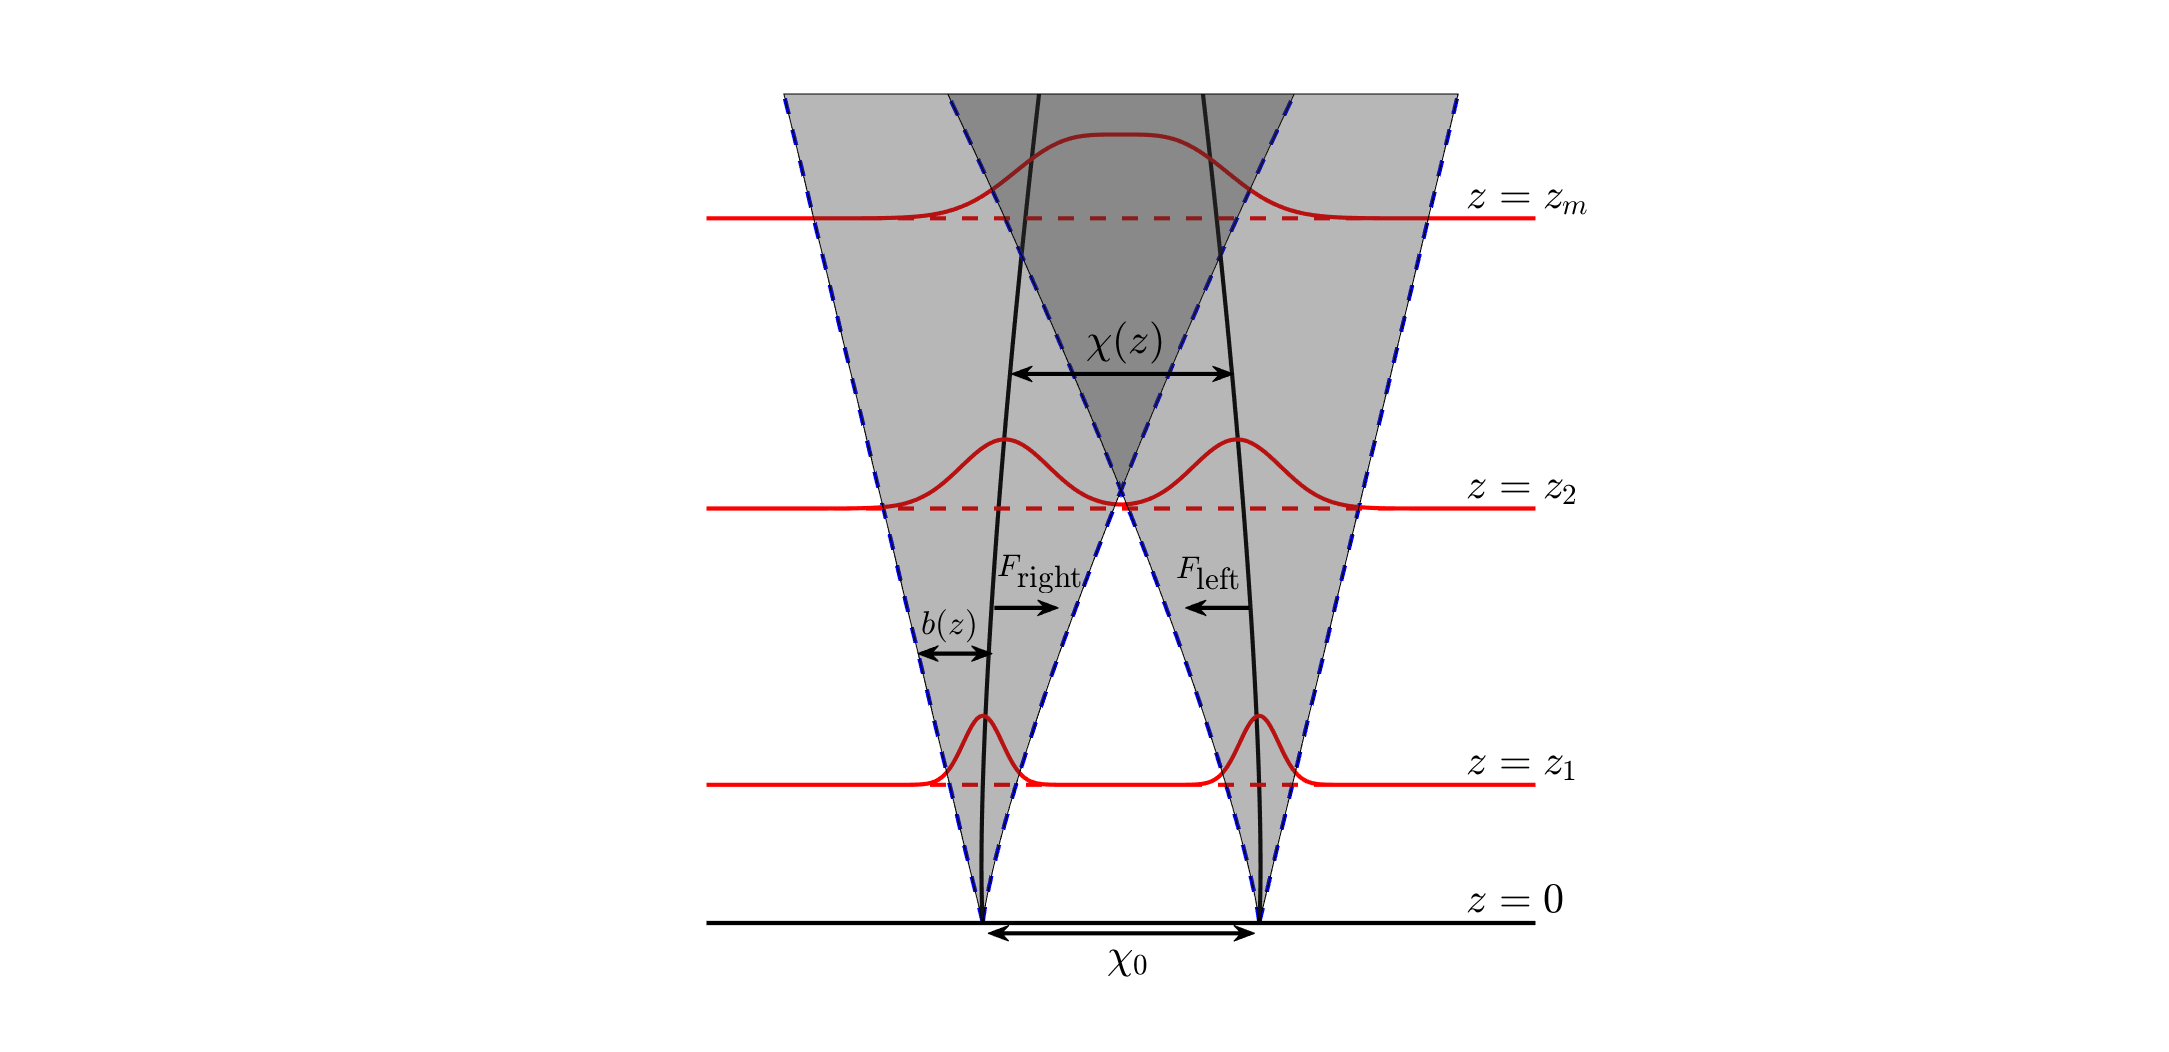
\includegraphics[trim = {9.5cm 1cm 9.5cm 1cm}, clip,width = 0.75\textwidth]{interactingTwoPlumeSchematic.eps}
		\caption{Schematic of two interacting plumes. The dashed blue lines show the edges of the plume, the solid black lines represent the centreline of the plumes and solid red lines show the Gaussian buoyancy profile at the height shown by the dashed red lines.}
		\label{fig:twoInteractingPlumesSchematic}
	\end{figure}
	\subsubsection{Two interacting plumes}
	Suppose that we consider two interacting plumes, which are separated by a distance $\chi_0$ and are both of equal strength. As in the non-interacting case, we configure these plumes WLOG such that the line is centred at $x = 0$. In this case, the sources of these plumes are at $(-\tfrac{1}{2}\chi_0,0), (\tfrac{1}{2}\chi_0,0)$. We model the centreline of these plumes as line sinks of buoyancy located at $(\chi_1,z),(\chi_2,z)$. As the plumes are of equal strength, by symmetry we have that $\chi_1 = -\chi_2$. The strength of these plumes are given by $m(z) = 2\pi\alpha b(z)w(z)$. The entrainment felt by one plume on another is given by $F = \tfrac{m}{2\pi}\tfrac{1}{r^{\prime}}$ where $r^{\prime}(z)$ is the distance between the centrelines of the two plumes at $z$. By symmetry, we take $\chi_2 = -\chi_1$. A schematic of this two plume case is given in figure \ref{fig:twoInteractingPlumesSchematic}. \\
	
	\noindent It was shown in KL04 that the rate of change of centreline separation between plumes as a function of height is given by the ratio between horizontal (entrainment) velocity and vertical velocity. That is
	\begin{equation}
	\dbyd{\chi_1}{z} = \frac{F_1}{w} \label{eqn:first interacting plume ODE}
	\end{equation}
	where 
	\begin{align}
	F_1 = b\alpha w \left(\frac{1}{\chi_2 - \chi_1}\right) = -\frac{b\alpha}{2\chi_1} \label{eqn:first plume contribution}
	\end{align}
	where $\chi_1(0) = -\tfrac{1}{2}\chi_0$ and $\chi_2 = -\chi_1$. 
	Solving this system of ODEs analytically, we see that
	\begin{align}
		\chi_1(z) = \left\{\frac{1}{4}\chi_0^2 - \frac{3}{5}\alpha^2z^2 \right\}^{1/2}, \quad \chi_2(z) = -\left\{\frac{1}{4}\chi_0^2 - \frac{3}{5}\alpha^2z^2 \right\}^{1/2}.
	\end{align}
	To determine the height at which these plumes have merged, we substitute this analytic solution into the formulation of $E$ given by
	\begin{eqnarray}
	\displaystyle{E(x,z) = \exp\left(- \left[\frac{x - \chi_1}{b}\right]^2 \right) + \exp\left(- \left[\frac{x - \chi_2}{b}\right]^2\right)} \label{eqn:interacting two plume buoyancy}
	\end{eqnarray}
	and determine the first height where $E$ has a single peak.
	By substituting the analytic solution for $\chi_1$ and $\chi_2$, the buoyancy profile is given by		
	\begin{eqnarray}
	\displaystyle{E(x,z) = \exp\left(- \left[\frac{x - (\frac{1}{4}\chi_0^2 - \frac{3}{5}\alpha^2z)^{1/2}}{\frac{6\alpha z}{5}}\right]^2 \right) + \exp\left(- \left[\frac{x + (\frac{1}{4}\chi_0^2 - \frac{3}{5}\alpha^2z)^{1/2}}{\frac{6\alpha z}{5}}\right]^2\right)}
	.\label{eqn:two plume interacting buoyancy profile}
	\end{eqnarray}
	Using peak detection in both Python and MATLAB, we find that the merging height is given by $\lambda_m^I = \tfrac{0.435}{\alpha}$ which is in excellent agreement with the analytic solution found independently in KL04, given by $\lambda_m^I = \tfrac{1}{\alpha}\sqrt{\frac{25}{132}}$. Furthermore, by solving \eqref{eqn:first interacting plume ODE} subject to \eqref{eqn:first plume contribution} and following the method above, we arrive an identical solution for the merging height.
	
	\subsubsection{Three interacting plumes}
	Suppose also that we have three interacting co-linear plumes, configured with sources at $(-\chi_0,0),(0,0),(\chi_0,0)$. We model these plumes as line sinks positions at $(\chi_1,z),(\chi_2,z),(\chi_3,z)$ where $\chi_2 = 0$ and $\chi_3 = -\chi_1$ by symmetry.
	Recall that the entrainment velocity of one plume on another is given by $F = b\alpha w \tfrac{1}{r^{\prime}}$ where $r^{\prime}$ is the centreline separation between the plumes at a given height. Therefore the entrainment velocity of plume 1, located at $(\chi_1,z)$ is given by
	\begin{equation}
		F_1 = b\alpha w\left(\frac{1}{\chi_3 - \chi_1} + \frac{1}{\chi_2 - \chi_1}\right) = \frac{-3b\alpha w}{2\chi_1}.
	\end{equation}
	Similarly, for plume 2, we see that
	\begin{equation}
		F_2 = b\alpha w \left(\frac{1}{\chi_3 - \chi_2} + \frac{1}{\chi_1 - \chi_2}\right) = 0
	\end{equation}
	and by symmetry about $x = 0$, we take $F_3 = -F_1$. For each plume, we assume that the change in centreline position with height is given by the ratio of horizontal to vertical velocity. This is expressed as
		\begin{eqnarray}
	\dbyd{\chi_k}{z} = \frac{F_k}{w}.
	\end{eqnarray}
	Explicitly, for three plumes, the system of equations are
	\begin{align}
	\dbyd{\chi_1}{z} &= -\frac{3b\alpha}{2\chi_1} \label{eqn:three plume ODE general plume 1}\\
	\dbyd{\chi_2}{z} &= 0 \label{eqn:three plume ODE general plume 2}\\
	\chi_3 &= -\chi_1 \label{eqn:three plume ODE general plume 3}
	\end{align}
	subject to $\chi_1(0) = -\chi_0, \chi_2(0) = 0$ and $\chi_3(0) = \chi_0$. Solving \eqref{eqn:three plume ODE general plume 1} - \eqref{eqn:three plume ODE general plume 3} analytically, we find that
	\begin{align}
	\chi_1 &= \left(\chi_0^2 - \frac{9\alpha^2}{5}z^2\right)^{\frac{1}{2}}\\
	\chi_2 &= 0 \\
	\chi_3 &= -\left(\chi_0^2 - \frac{9\alpha^2}{5}z^2\right)^{\frac{1}{2}}.
	\end{align}
	From this analytic solution, we determine the buoyancy profile, $E$, defined by
	\begin{eqnarray}
	\begin{split}
	E(x,z) &= \exp\left(- \left[\frac{x - \chi_1}{b}\right]^2 \right) + \exp\left(- \left[\frac{x - \chi_2}{b}\right]^2\right) \\
	&+ \exp\left(- \left[\frac{x - \chi_3}{b}\right]^2\right).
	\end{split} \label{eqn:interacting three plume buoyancy}
	\end{eqnarray}
	By substituting the analytic solution for $\chi_1,\chi_2$ and $\chi_3$, the buoyancy profile is given by		
	\begin{eqnarray}
	\begin{split}
	E(x,z) &= \exp\left(- \left[\frac{x - (\chi_0^2 - \frac{9\alpha^2z}{5})^{1/2}}{\frac{6\alpha z}{5}}\right]^2 \right) + \exp\left(- \left[\frac{x}{\frac{6\alpha z}{5}}\right]^2\right) \\
	&+ \exp\left(- \left[\frac{x + (\chi_0^2 - \frac{9\alpha^2z}{5} )^{1/2}}{\frac{6\alpha z}{5}}\right]^2\right).\label{eqn:three plume interacting buoyancy profile}
	\end{split}
	\end{eqnarray}	
	The merging height of this system is found by applying the method outlined in \S\ref{subsec:odd line of NI plumes}. We find that $\lambda_m^I \alpha = 0.454$. We may also solve \eqref{eqn:three plume ODE general plume 1} - \eqref{eqn:three plume ODE general plume 3} numerically. By doing so, and determining the number of peaks given in \eqref{eqn:interacting three plume buoyancy}, we further validate this model by arriving at a merging height of $\lambda_m^I\alpha = 0.454$, as expected from the analytic solution.
	
	\subsubsection{An odd number of co-linear plumes}
	Suppose that we have $n$, where $n$ is odd, interacting co-linear plumes, configured such that the line is centred about $x = 0$. This requires the plumes to be centred at 
	$$\left(-\dfrac{n-1}{2}\chi_0,0\right), \left(-\dfrac{n-3}{2}\chi_0,0\right), \dots, (0,0), \dots, \left(\dfrac{n-1}{2}\chi_0,0\right). $$
	This is modelled as a line of $n$ line sinks of strength $-m(z)$ at 
	$$\left(\chi_1,z\right), \left(\chi_2,z\right), \dots, \left(\chi_{(n+1)/2},z\right), \dots, \left(\chi_n,z\right).$$
	These plumes are labelled, left to right, as plume 1,2,...$n$. For plume 1, we see that the entrainment velocity is given by 
	\begin{align}
	F_1 &= \displaystyle{b\alpha w \left( \frac{1}{\chi_n - \chi_1} + \frac{1}{\chi_{n-1} - \chi_1} + \dots \frac{1}{\chi_2 - \chi_1}\right)}\\
	&= b\alpha w \displaystyle{\sum_{j=2}^{n} \frac{1}{\chi_j - \chi_1}}
	\end{align}
	
	For an arbitrary plume number, $k$, where $1<k\leq \tfrac{n-1}{2}$ we find that the entrainment velocity is given by
	\begin{align}
	F_k &= b\alpha w \displaystyle{ \left(\frac{1}{\chi_n - \chi_k} + \dots + \frac{1}{\chi_{k+1} - \chi_k} - \left[\frac{1}{\chi_k - \chi_{k-1}} + \dots \frac{1}{\chi_k - \chi_1}\right]\right)}\\
	&= b\alpha w \left( \underbrace{\sum_{j=k+1}^{n} \frac{1}{\chi_j - \chi_k}}_{\text{right of $k^{th}$ plume}}  - \underbrace{\sum_{j=1}^{k-1}\frac{1}{\chi_k - \chi_j}}_{\text{left of $k^{th}$ plume}}\right) \label{eqn:general odd entrainment velocity} \\
	& = b\alpha w \sum_{\substack{j=1\\ j\neq k}}^{n} \frac{1}{\chi_j - \chi_k}. \label{eqn:general odd entrainment velocity concise}
	\end{align}
	By the symmetry of the system, we also have $\chi_n = -\chi_1$, $\chi_{n-1} = - \chi_2$ and in general $\chi_{n-k+1} = -\chi_k$ for $k \leq \frac{n-1}{2}$. Finally, $\chi_{(n+1)/2} = 0$, again by the symmetry of the configuration. This yields the following system of equations 
	\begin{align}
	\dbyd{\chi_k}{z} &= \frac{F_k}{w} \quad \text{for $1\leq k \leq \frac{n-1}{2}$} \label{eqn:general odd plume merging ODE left}\\
	\chi_k &= 0 \quad \text{for $k = \frac{n+1}{2}$} \label{eqn:general odd plume merging ODE centre} \\
	\chi_k &= -\chi_{n+1-k} \quad \text{for $\frac{n+3}{2}\leq k \leq n$}\label{eqn:general odd plume merging ODE right}
	\end{align}
	subject to $\chi_k(0) = -\left(\frac{n-(2k-1)}{2}\right)\chi_0$. 
	The system of equations given by \eqref{eqn:general odd plume merging ODE left} - \eqref{eqn:general odd plume merging ODE right} can be solved numerically to give the centreline of each plume as a function of height. There will not, in general, be an analytic solution for these centrelines, so the merging height can not be found using the method outlined in REF. Instead, the buoyancy profile, $E$, is computed and the number of peaks found using MATLAB peak detection. Once this number of peaks has reduced from $n$ to 1, the system of plumes has merged, and the lowest height for which this is seen is the merging height, $z_m^I$. This merging height may then be non-dimensionalised as previously, to give $\lambda_m^I = \frac{z_m^I}{\chi_0}$.\\
	
	\noindent However this model overlooks the physical behaviour of the system. Implicit in this model is the assumption that the plumes all merge simultaneously, at the same height. While this is true for $n = 3$, this isn't the case in general. Instead, we see that the outer two plumes merge first (that is, plumes 1 and 2 merge, as do plumes $n-1$ and $n$), then these merged plumes merge with the adjacent plume and so on until a single plume remains. Furthermore, the strength of these merged plumes is no longer the same as the plumes that have yet to merge. Indeed, in REF, it was shown that the radius of the merged plume at the merging height, $b_m$, increases with the number of plumes that have merged. Explicitly, we showed that $b_m = \sqrt{n}b$, where $b$ is the radius of an ``unmerged'' plume at the merging height. \\
	
	\noindent Therefore, we initially have $n$ equal co-linear plumes. These $n$ plumes will merge into $n-2$ because plumes 1 and 2 have merged, as have plumes $n$ and $n-1$. Each merged plume is $\sqrt{2}$ times stronger than each of the remaining $n-2$ plumes (see \S \ref{subsubsec:Physical quantities} or KL04). Hence, we must consider the merging behaviour of non-equal plumes. \\
	
	\noindent Consider two plumes, with specific buoyancy fluxes $F_1$ and $F_2$, where $F_1\geq F_2 \, \forall z$. We define the ratio of fluxes, $\psi = \frac{F_2}{F_1} \leq 1$. It was shown, in KL04, that the buoyancy profile of two non-equal plumes is given by
	\begin{equation}
		E(x,z,\psi) = \exp\left(-\left[\frac{x-\chi_1}{b_1}\right]^2\right) + \psi^{\frac{2}{3}}\exp\left(-\left[\frac{x-\chi_2}{b_2}\right]^2\right)\label{eqn:two non-equal plumes buoyancy profile}
	\end{equation}
	where subscripts $1$ and $2$ refer to the values of these quantities on plumes 1 and 2 respectively. When $\psi = 1$, we return to the equal plume case as expected. \\
	
	\noindent The buoyancy profile given in \eqref{eqn:two non-equal plumes buoyancy profile} may be readily extended to $n$ non-equal plumes, where $k$ of these plumes have specific buoyancy flux $F_1$, and $n-k$ have specific buoyancy flux $F_2$, where $\tfrac{F_2}{F_1} = \psi \leq 1$. This more general buoyancy profile is given by	
	\begin{align}
		\begin{split}
			E(x,z,\psi) &= \sum_{j=1}^{k/2}\exp\left(-\left[\frac{x - \chi_j}{b_1}\right]^2\right) + \psi^{\frac{2}{3}}\sum_{j=\frac{k}{2}+1}^{n+1-\frac{k}{2}}\exp\left(-\left[\frac{x - \chi_j}{b_2}\right]^2\right) \\
			&+\sum_{j=n+2-\frac{k}{2}}^{n}\exp\left(-\left[\frac{x - \chi_j}{b_1}\right]^2\right)
		\end{split}
	\end{align}
	where $b_1 = \sqrt{\tfrac{1}{\psi}}b_2$. Note that the first sum corresponds to the merged plumes on the left side of the line of plumes, the third corresponds to the merged plumes on the right, and the second to the ``unmerged'' central plumes. Taking $k = 2$, we return to the case discussed above (provided that $n$ is odd). An example will be given for $n = 5$, and we note that the details may be extended to an arbitrary odd number of plumes.\\
	
	\noindent To compute the merging height for $n = 5$, we begin with five equal plumes. Labelling the centrelines of these plumes $\chi_1, \chi_2,\dots,\chi_5$ where $\chi_3 = 0$, $\chi_4 = -\chi_2$ and $\chi_5 = -\chi_1$ by symmetry. First, we consider the change in the centreline of the first plume. Using \eqref{eqn:general odd entrainment velocity concise} and \eqref{eqn:general odd plume merging ODE left} with $k = 1$, we see that
	\begin{equation}
		\dbyd{\chi_1}{z} = b\alpha \left[ \frac{1}{\chi_5 - \chi_1} + \frac{1}{\chi_4 - \chi_1} + \frac{1}{\chi_3 - \chi_1} + \frac{1}{\chi_2 - \chi_1} \right]\label{eqn:five plumes leftmost plume full form}.
	\end{equation}
	By applying the symmetry conditions: $\chi_3 = 0, \chi_4 = -\chi_2$ and $\chi_5 = -\chi_1$, \eqref{eqn:five plumes leftmost plume full form} reduces to 
	\begin{align}
		\dbyd{\chi_1}{z} &= b\alpha \left[\frac{1}{-\chi_1 - \chi_1} + \frac{1}{-\chi_2 - \chi_1} + \frac{1}{-\chi_1} + \frac{1}{\chi_2 - \chi_1}\right] \\
		&= b\alpha\left[-\frac{3}{2\chi_1} - \frac{1}{\chi_2 + \chi_1} + \frac{1}{\chi_2 - \chi_1}\right]
	\end{align}
	subject to $\chi_1(0) = -2\chi_0$.
	Similarly, for the second plume, we see that
	\begin{align}
		\dbyd{\chi_2}{z} &= b\alpha \left[\frac{1}{\chi_5 - \chi_2} + \frac{1}{\chi_4 - \chi_2} + \frac{1}{\chi_3 - \chi_2} + \frac{1}{\chi_1 - \chi_2}\right]\\
		&= b\alpha \left[\frac{1}{-\chi_1 - \chi_2} + \frac{1}{-\chi_2 - \chi_2} + \frac{1}{-\chi_2} + \frac{1}{\chi_1 - \chi_2}\right] \\
		&= b\alpha \left[-\frac{3}{2\chi_2} - \frac{1}{\chi_2 + \chi_1} - \frac{1}{\chi_2 - \chi_1}\right]
	\end{align}
	subject to $\chi_2(0) = -\chi_0$.
	With five plumes, the system of equations describing the location of the centrelines, $\chi_j$ for $j = 1,2,\dots 5$ are given by
	\begin{align}
		\dbyd{\chi_1}{z} &= b\alpha\left[-\frac{3}{2\chi_1} - \frac{1}{\chi_2 + \chi_1} + \frac{1}{\chi_2 - \chi_1}\right] \\
		\dbyd{\chi_2}{z} &= b\alpha \left[- \frac{3}{2\chi_2} - \frac{1}{\chi_2+\chi_1}-\frac{1}{\chi_2-\chi_1} \right] \\
		\chi_3 &= 0 \\
		\chi_4 &= -\chi_2 \\
		\chi_5 &= -\chi_1
	\end{align} 
	subject to $\chi_k(0) = -\frac{n-(2k-1)}{2}\chi_0$. This system of equations is solved using a forward Euler spatial stepping, and the buoyancy profile
	\begin{equation}
		E(x,z) = \sum_{j=1}^{5}\exp\left(-\left[\frac{x-\chi_j}{b}\right]^2\right)\label{eqn:five plumes buoyancy}
	\end{equation}
	computed until \eqref{eqn:five plumes buoyancy} has three peaks, instead of five. Suppose that this first occurs at $z = z_1$. We now have three plumes of non-equal strength which we label 1, 2, 3 and their centrelines $\bar{\chi_1}, \bar{\chi_2}, \bar{\chi_3}$ respectively. As plume 1 now contains two of the initial plumes (the previous plumes 1 and 2), and similarly plume 3, these new plumes have twice the buoyancy flux of the new plume 2. The ODE describing the location of $\bar{\chi_1}$ is given by
	\begin{align}
		\dbyd{\bar{\chi_1}}{z} &= \frac{b_3\alpha}{\bar{\chi_3}-\bar{\chi_1}} + \frac{b_2\alpha}{\bar{\chi_2}-\bar{\chi_1}} \\
		&= \frac{b_1\alpha}{-2\bar{\chi_1}} + \frac{b_2\alpha}{-\bar{\chi_1}}
	\end{align}
	subject to $\bar{\chi_1}(z_1) = \frac{1}{2}\left(\chi_1 + \chi_2\right)\vert_{z=z1}$ and $b_1 = \sqrt{2}b_2$. We also apply $\bar{\chi_2} = 0$ and $\bar{\chi_3} = -\bar{\chi}_1$. For this intermediate line of plumes, the buoyancy profile is given by
	\begin{equation}
		E(x,z) = \exp\left(-\left[\frac{x-\bar{\chi_1}}{b_1}\right]^2\right)
		+ \left(\frac{1}{2}\right)^{\frac{2}{3}}\exp\left(-\left[\frac{x}{b_2}\right]^2\right)
		+ \exp\left(-\left[\frac{x-\bar{\chi_3}}{b_1}\right]^2\right). \label{eqn:three plumes nonequal buoyancy profile}
	\end{equation}
	\\
	\noindent Iteratively solving for $\bar{\chi_1}$, applying the symmetry conditions for $\bar{\chi_2}$ and $\bar{\chi_3}$, we determine \eqref{eqn:three plumes nonequal buoyancy profile} for each $z$. The merging height of the line of five plumes is then given by the first height $z$ for which \eqref{eqn:three plumes nonequal buoyancy profile} has a single peak. This single peak is found using MATLAB peak detection. We find that, for $n = 5$, the merging height is given by $\lambda_m^I \alpha = 0.55$.
	\subsubsection{An even number of co-linear plumes}
	The interacting case for a line of an even number of plumes is also configured such that the line of plumes is centred about $x = 0$. This is done by centring the plumes at 
	$$(x,z) = \left(-\dfrac{n-1}{2}\chi_0,0\right), \dots, \left(-\dfrac{n-(2k-1)}{2}\chi_0,0\right), \dots, \left(\dfrac{n-1}{2}\chi_0,0\right).$$
	Therefore, I model this as line sinks placed at 
	$$x = \chi_1, \dots,\chi_k, \dots, \chi_n.$$
	However, we note that this configuration does not have a plume source located at $x = 0$. That is, the midpoint of the configuration is not necessarily a maximum, and won't be until the line of plumes has merged. Instead of the intial system of equations given by \eqref{eqn:general odd plume merging ODE left} - \eqref{eqn:general odd plume merging ODE right}, the initial system  is given by
	\begin{align}
		\dbyd{\chi_k}{z} = \frac{F_k}{w} \quad \text{for $1\leq k \leq \frac{n}{2}$} \\
		\chi_{k} = -\chi_{n-k+1} \quad \text{for $\frac{n}{2}+1 \leq k \leq n$}
	\end{align}
	where $F_k$ is given by \eqref{eqn:general odd entrainment velocity}.
	From here, the method is identical to the odd case.  Example outputs for four and five co-linear plumes are given in figure \ref{fig:four and five output}.
	
	\begin{figure}
		\begin{overpic}[width = 0.5\textwidth]{fourPlumesInteracting.eps}
			\put(0,45){$\lambda$}
			\put(44,0){$x/\chi_0$}
		\end{overpic}
		\hfill 
		%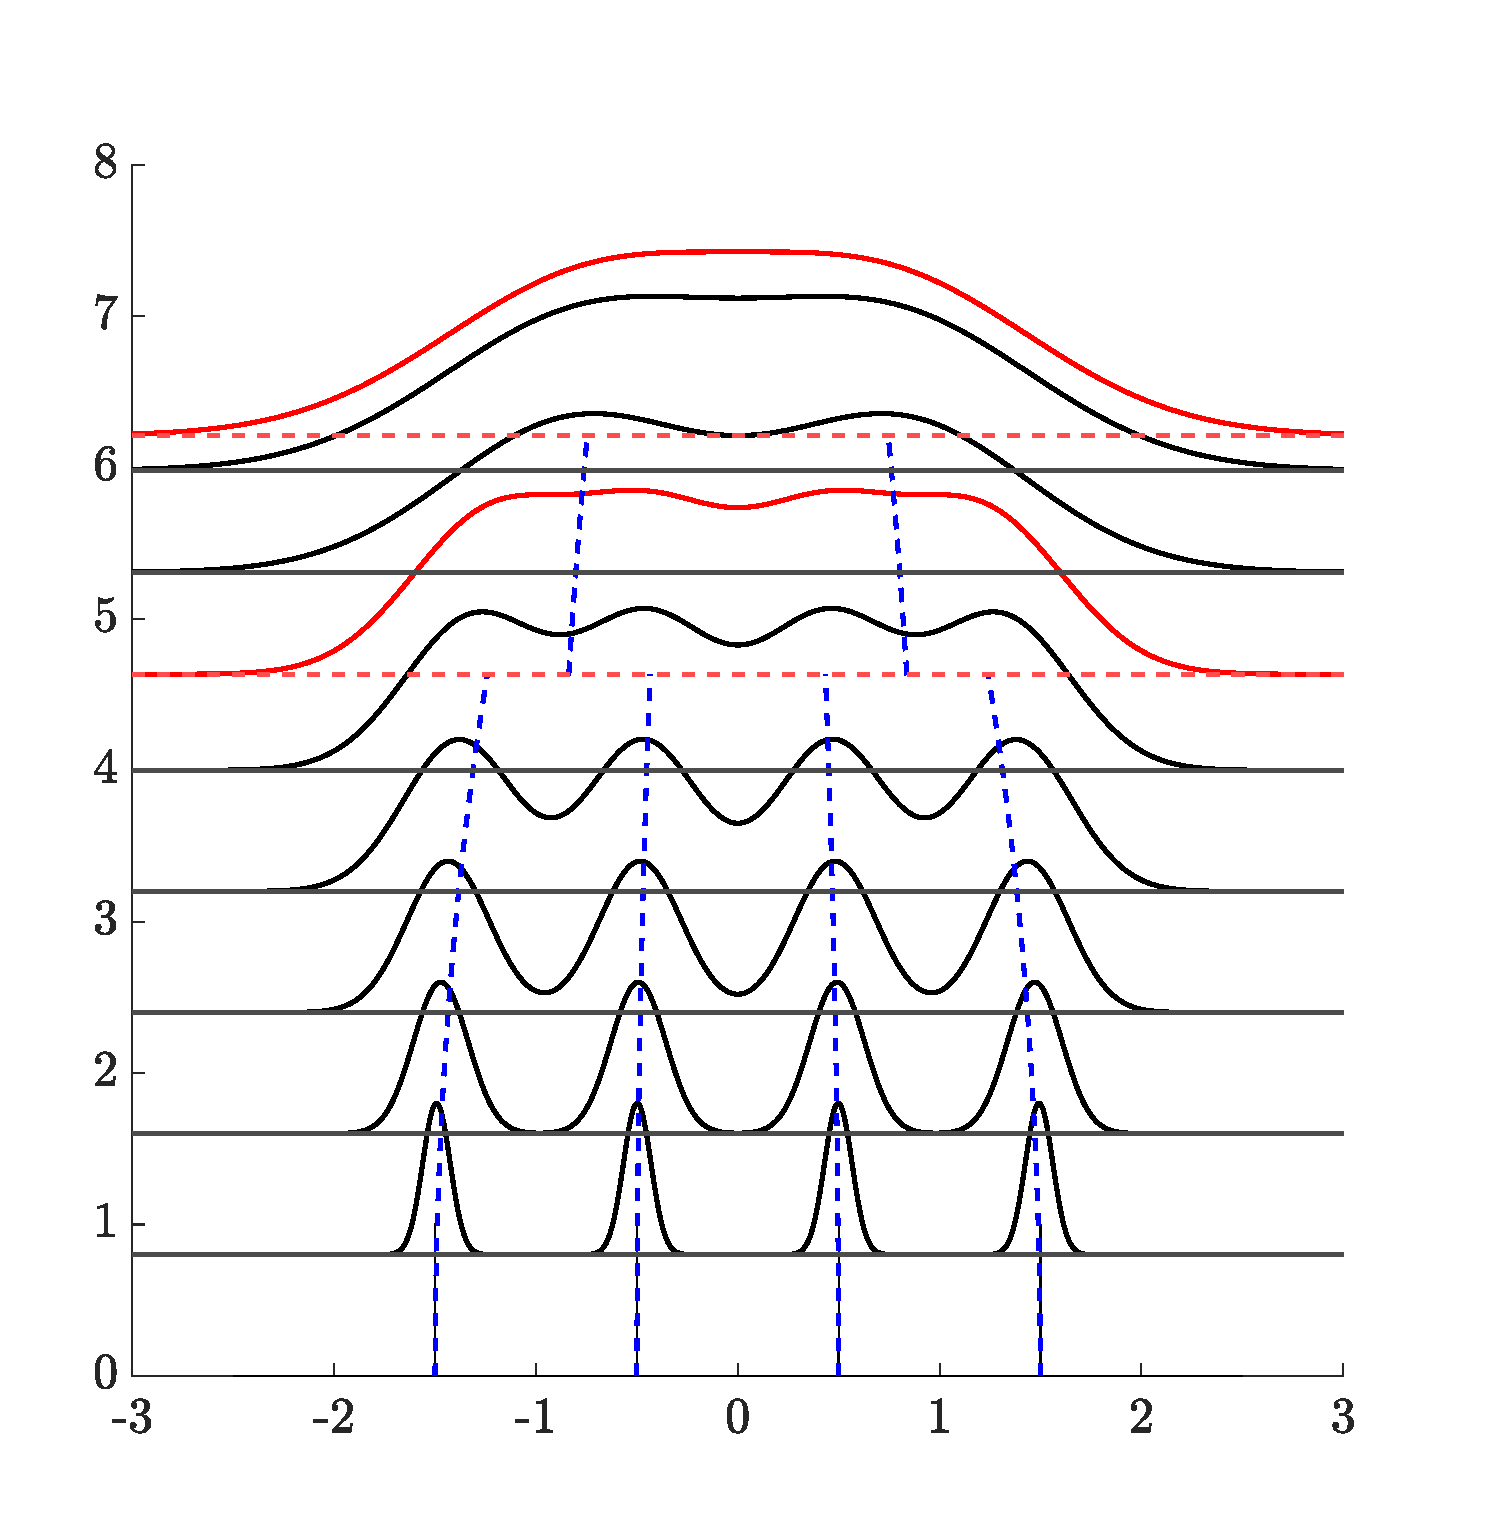
\includegraphics[width = 0.475\textwidth]{fourPlumesInteracting.eps}\hfill
		\begin{overpic}[width = 0.5\textwidth]{fivePlumesInteracting.eps}
			\put(0,45) {$\lambda$}
			\put(43,0){$x/\chi_0$}
		\end{overpic}
		\caption{Example outputs for $n = 4$ (left) and $n = 5$ plumes (right) with $\alpha = 0.1$. The heights at which the number of plumes decreases from four to two to one (or five to three to one) are shown in red.}
		\label{fig:four and five output}
	\end{figure}

	\subsection{Arrays of interacting plumes}
	Extend the late game model to an extra dimension and give componentwise merging to give interacting merging heights for the following two cases.
	\subsubsection{An equilateral triangle}
		\begin{figure}
			\centering
			\includegraphics[width = 0.65\textwidth]{triangularSchematicNI.png}	
			\caption{Schematic of an equilateral triangle of interacting plumes.}
			\label{fig:interacting triangle}
		\end{figure}
	We consider an equilateral triangle of interacting plumes where each plume has the same strength. This configuration is given in figure \ref{fig:interacting triangle}. From this schematic, we see that each plume is entrained by two others. We extend the method outlined in $\S$ \ref{subsec:Line of interacting plumes} as follows: denote the location of the centreline of the $k^{\text{th}}$ plume by $\mathbf{\chi}_k = (\chi_{k,i},\chi_{k,j})$. We then assume that the merging in each direction is independent, i.e. that the merging in the $x$ direction is independent of that in the $y$. We then formulate ODEs for each component of each centreline. \\
	
	\noindent Consider a triangular array with sources located at $\left(-\frac{1}{2}\chi_0,0\right)$, $\left(\frac{1}{2}\chi_0,0\right)$ and $\left(0,\frac{\sqrt{3}}{2}\chi_0\right)$. Labelling the plumes located at the above positions as $\mathbf{\chi}_1$, $\mathbf{\chi}_2$ and $\mathbf{\chi}_3$ respectively, we generate the following system of equations
	\begin{align}
		\dbyd{}{z} \left(\chi_{1,i}\right) &= b\alpha \left[\frac{1}{\chi_{3,i} - \chi_{1,i}} + \frac{1}{\chi_{2,i}-\chi_{1,i}} \right] \\
		\dbyd{}{z} \left(\chi_{1,j}\right) &= b\alpha \left[\frac{1}{\chi_{3,j}-\chi_{1,j}}\right] \\
		\chi_{2,i} &= -\chi_{1,i} \quad\text{\small due to symmetry about $x = 0$}\\
		\chi_{2,j} &= \chi_{1,j} \quad\text{\small as these centrelines are in the same vertical plane}\\
		\chi_{3,i} &= 0 \quad \text{\small by symmetry about $x = 0$}\\
		\dbyd{}{z}\left(\chi_{3,j}\right) &= b\alpha\left[\frac{2}{\chi_{1,j}-\chi_{3,j}}\right]
	\end{align}
	subject to $\left(\chi_{1,i},\chi_{1,j}\right)\vert_{z=0} = \left(-\frac{1}{2}\chi_0,0\right)$, $\left(\chi_{2,i},\chi_{2,j}\right)\vert_{z=0} = \left(\frac{1}{2}\chi_0,0\right)$ and $\left(\chi_{3,i},\chi_{3,j}\right)\vert_{z=0} = \left(0,\frac{\sqrt{3}}{2}\chi_0\right)$. \\
		
	\noindent By solving the above system of equations, we capture the behaviour of each centreline in both $x$ and $y$ directions. We then define a buoyancy function, extended to an additional spatial dimension, given by
	
	\begin{equation}
		E(x,y,z) = \sum_{k=1}^{3} \exp\left(- \left[\frac{(x - \chi_{k,i})^2 + (y - \chi_{k,j})^2}{b(z)^2}\right]\right). \label{eqn:array buoyancy profile}
	\end{equation}
	\\
	\noindent As in REF, we seek the first height at which equation has a single peak. For a 2D array, the surface given by \eqref{eqn:array buoyancy profile} is plotted, and the number of peaks of this surface are determined using peak detection. \eqref{eqn:array buoyancy profile} is plotted iteratively until the first height of a single peak is determined. This is the merging height, $\lambda_m^I$, of the triangular array of plumes and is found to be $\lambda_m^I = \frac{0.318}{\alpha}$.
	\subsubsection{2 $\times$ 2 grid}
	Finally, we consider a $2 \times 2$ grid of plumes, where the sides of the grid are $\chi_0$ and therefore the diagonal distance between corners is $\sqrt{2}\chi_0$. Labelling the corners of the square, starting in the bottom left, anti-clockwise as 1,2,3 and 4, the plume sources are given by $\displaystyle{\left(\chi_{1,i},\chi_{1,j}\right)\vert_{z=0} = \left(-\frac{1}{2}\chi_0,-\frac{1}{2}\chi_0\right)}$, $\displaystyle{\left(\chi_{2,i},\chi_{2,j}\right)\vert_{z=0} = \left(\frac{1}{2}\chi_0,-\frac{1}{2}\chi_0\right)}$, $\displaystyle{\left(\chi_{3,i},\chi_{3,j}\right)\vert_{z=0} = \left(\frac{1}{2}\chi_0,\frac{1}{2}\chi_0\right)}$ and $\displaystyle{\left(\chi_{4,i},\chi_{4,j}\right)\vert_{z = 0} = \left(-\frac{1}{2}\chi_0,\frac{1}{2}\chi_0\right)}$.\\
	
	\noindent As in ref, we formulate a system of equations to describe the centrelines of the plumes in this grid, given by
	\begin{align}
		\dbyd{}{z}\left(\chi_{1,i}\right) & = b\alpha\left[\frac{1}{\chi_{3,i}-\chi_{1,i}} + \frac{1}{\chi_{2,i} - \chi_{1,i}}\right] \\
		\dbyd{}{z}\left(\chi_{1,j}\right) & = b\alpha\left[\frac{1}{\chi_{4,j}-\chi_{1,j}} + \frac{1}{\chi_{3,j} - \chi_{1,j}}\right]	\\
		\chi_{2,i} &= -\chi_{1,i} \\
		\chi_{2,j} &= \chi_{1,j} \\
		\chi_{3,i} &= \chi_{2,i} \\
		\chi_{3,j} &= -\chi_{1,j} \\
		\chi_{4,i} &= \chi_{1,i} \\
		\chi_{4,j} &= \chi_{3,j}
	\end{align}
	subject to the above initial conditions, shown in figure \ref{fig:interacting grid}. 
	\begin{figure}
		\begin{picture}(\textwidth,0.65\textwidth)
			\centering
			\linethickness{1.5pt}
			\put(3cm,2cm){\line(1,0){6cm}}
			\put(3cm,2cm){\line(0,1){6cm}}
			\put(9cm,2cm){\line(0,1){6cm}}	
			\put(3cm,8cm){\line(1,0){6cm}}
			
			\put(3cm,2cm){\circle{10}}
			\put(3cm,2cm){\color{red}\circle*{10}}
			\put(2cm,1.4cm){$\left(-\frac{1}{2}\chi_0,-\frac{1}{2}\chi_0\right)$}
			\put(3.25cm,2.25cm){\color{blue} 1}
			
			\put(9cm,2cm){\circle{10}}
			\put(9cm,2cm){\color{red}\circle*{10}}	
			\put(8cm,1.4cm){$\left(\frac{1}{2}\chi_0,-\frac{1}{2}\chi_0\right)$}
			\put(8.5cm,2.25cm){\color{blue} 2}
			
			\put(9cm,8cm){\circle{10}}
			\put(9cm,8cm){\color{red}\circle*{10}}
			\put(8cm,8.4cm){$\left(\frac{1}{2}\chi_0,\frac{1}{2}\chi_0\right)$}
			\put(8.5cm,7.5cm){\color{blue} 3}
			
			\put(3cm,8cm){\circle{10}}
			\put(3cm,8cm){\color{red}\circle*{10}}
			\put(2cm,8.4cm){$\left(-\frac{1}{2}\chi_0,\frac{1}{2}\chi_0\right)$}
			\put(3.25cm,7.5cm){\color{blue} 4}
		\end{picture}
		\vspace{-10ex}
		\caption{Schematic of the $2 \times 2$ array of interacting plumes.}
		\label{fig:interacting grid}
	\end{figure}
	The buoyancy profile is then given by
	\begin{equation}
		E(x,y,z) = \sum_{k=1}^{4} \exp\left(- \left[\frac{(x - \chi_{k,i})^2 + (y - \chi_{k,j})^2}{b(z)^2}\right]\right).
	\end{equation}
	By determining the first height at which equation has a single peak, we find the merging height $\lambda_m^I = \frac{0.361}{\alpha}$.
	
	\section{Experimental data}
	The modelling work of $\S$\ref{sec:non-interacting plumes}  and $\S$\ref{sec:Interacting Plumes} aimed to find a non-dimensional height at which a line, or array, of plumes will behave as as single, larger plume. This height is defined as the merging height or height of coalescence. We experimentally find this merging height, and compare to the values predicted by the interacting and non-interacting models. The notation of KL04 is used to allow for direct comparison. We denote the experimental merging height by $z_{\text{me}}$, and the corresponding experimental, non-dimensional merging height by $\lambda_{\text{me}}$. Recall also that the non-dimensional merging heights from the non-interacting and interacting models are given by $\lambda_{m}^{NI}$ and $\lambda_{m}^I$ respectively.
	
	\subsection{Set up and technique}
	Experiments were performed in a perspex tank with dimenions 750\,mm $\times$ 650\,mm $\times$  650\,mm. This tank was filled with freshwater of density $\rho = 1000\,\text{kg\,m}^{-3}$, which was measured by a sodium chloride refractometer. The plumes were created using a saline solution of density $\rho = 1033\,\text{kg\,m}^{-3}$, again measured with a sodium chloride refractometer. This solution was created using 20 litres of freshwater mixed thoroughly with 1.03\,kg of sodium chloride. The plumes were visualised using 3 grams of E151 brilliant black dye and 0.3 grams of yellow tartrazine dye.\\

	\noindent The footage was collected at 30 frames per second using a camera with a 25\,mm lens. To ensure constant lighting, a uniform intensity light sheet was placed behind the perspex tank. All other light sources were removed from the laboratory. This was done to remove ``noise’’ from the data. The experimental set up is given schematically in figure \ref{fig:L2Schematic}.
    \begin{figure}
		\centering
		\includegraphics[width=\textwidth]{L2Schematic.png}
		\caption{ Schematic of the experimental set up used for the merging plumes in a stationary environment experiments.}
		\label{fig:L2Schematic}
	\end{figure} 
	To ensure that the plumes created were fully turbulent, a set of four custom plume nozzles were created following the design by Dr Paul Cooper, Department of Mechanical Engineering, University of Wollongong, NSW, Australia.\\
	
	\noindent Due to the number of plume nozzles available, we performed experiments with a single plume and lines of two, three and four plumes, an equilateral triangle array and a 2 $\times$  2 square array. Each of these plumes has the same strength, and all lines of plumes are configured such that each plume is separated by the same distance from its nearest neighbour. \\
	
	\noindent Single plume experiments were performed to determine the entrainment coefficient of each nozzle. We then performed experiments focused on merging heights. The method for these experiments is given as follows:
	
	\begin{enumerate}
		\item Set the nozzle separation (skip this step for an experiment using only one nozzle).
		\item Fill the perspex tank to 700\,mm with freshwater. Ensure that the tank has no internal flow before continuing. This is achieved, based on preliminary experimentation, by waiting approximately 45 minutes between the end of filling and the start of the experiment.
		\item By very carefully running a long thin sponge along the front glass panel, so as not to introduce an internal flow, remove any bubbles from the front of the perspex tank. If currents were present, the experimental was delayed until they ceased.
		\item Record 300 frames of background footage. This was used later to remove background noise from plume imagery (explained later in REF).
		\item Turn on all nozzles being used and allow to run for 30 seconds. This allows the plume(s) to establish.
		\item Begin recording the experiment. Record for 45 seconds.
		\item Stop recording, turn off nozzles and drain the water from the perspex tank.
		\item Increase the nozzle separation by 5\,mm. Repeat method until the configuration no longer merges before reaching the bottom of the tank.
	\end{enumerate}
	\subsection{Data processing}\label{subsec:Data processing}
	The footage captured in these plume experiments must be processed to determine the merging height. We first performed the dye attenuation technique, outlined in CITE, in Digiflow (documentation found at \url{http://www.dampt.cam.ac.uk/lab/digiflow/}). The background image is subtracted from each frame of the recorded footage. We then time-average these frames to give the processed, time-averaged, plume configuration behaviour in a single image. An example of this technique is given in figure \ref{fig:dyeAttenuation}. This is done because the modelling in $\S$\ref{sec:non-interacting plumes}  and $\S$\ref{sec:Interacting Plumes} only considers steady plumes. An example of instantaneous behaviour is given in figure \ref{fig:instant snapshots}, and the time-averaged behaviour is given in figure \ref{fig:averaged images}. \\
	
	The entrainment coefficient must also be determined. Recall that the radius of a steady plume is given by $b = \tfrac{6\alpha}{5}z$ for height $z$ and entrainment coefficient $\alpha$. Therefore, by computing the radius of a single plume from the experimental data, we determine $\alpha$. Doing so, the entrainment cofficient is determined to be $\alpha = 0.086$. \\
	
	These experiments also require a virtual origin correction. The experiments were performed using a nozzle radius ($b_0$) of 2.5\,mm, an initial velocity ($w_0$) of $0.088\,\text{m\,s}^{-1}$ and a modified gravity ($g_0^{\prime}$) of $0.392\,\text{m\,s}{-2}$. This results in a source Froude number $\Gamma_0 = 0.921$ and therefore a virtual origin correction of 2.10\,cm was used.
	\begin{figure}
		\centering 
		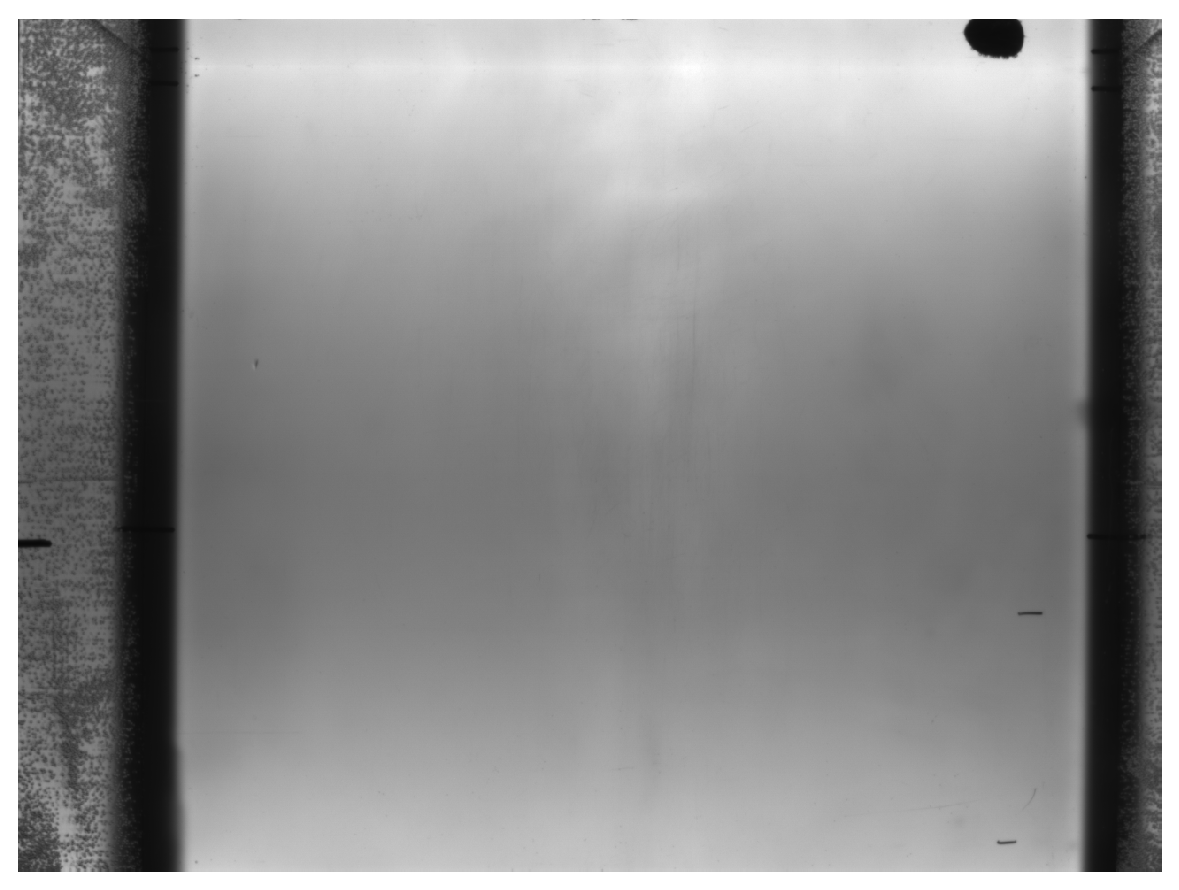
\includegraphics[trim = {0cm 0cm, 0cm, 0cm}, clip,width=0.45\textwidth,height = 2.6in,angle = 180]{frame650BG.eps}
			%\includegraphics[trim = {6.5cm 0cm 4.5cm 0cm}, clip,width = 0.65\textwidth, keepaspectratio]{background.eps}
		\hspace{1em}
		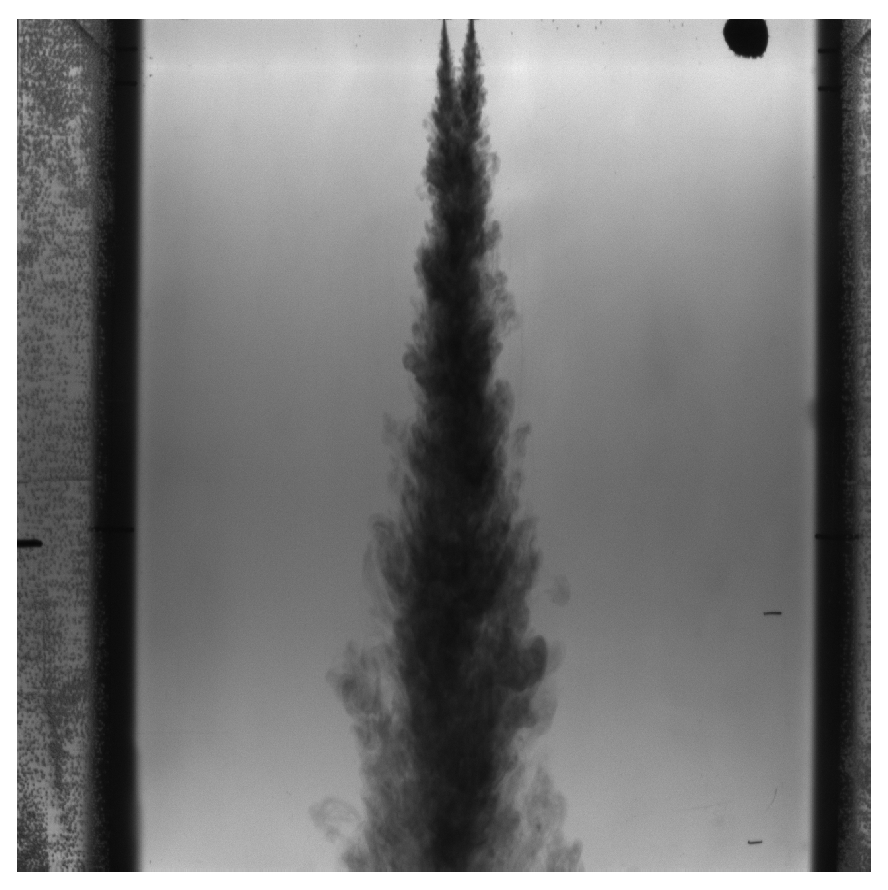
\includegraphics[trim = {0 0cm 0cm 0}, clip,width=0.45\textwidth, height = 2.6in,angle = 180]{frame650.eps}
		
		\vspace{0.5em}
		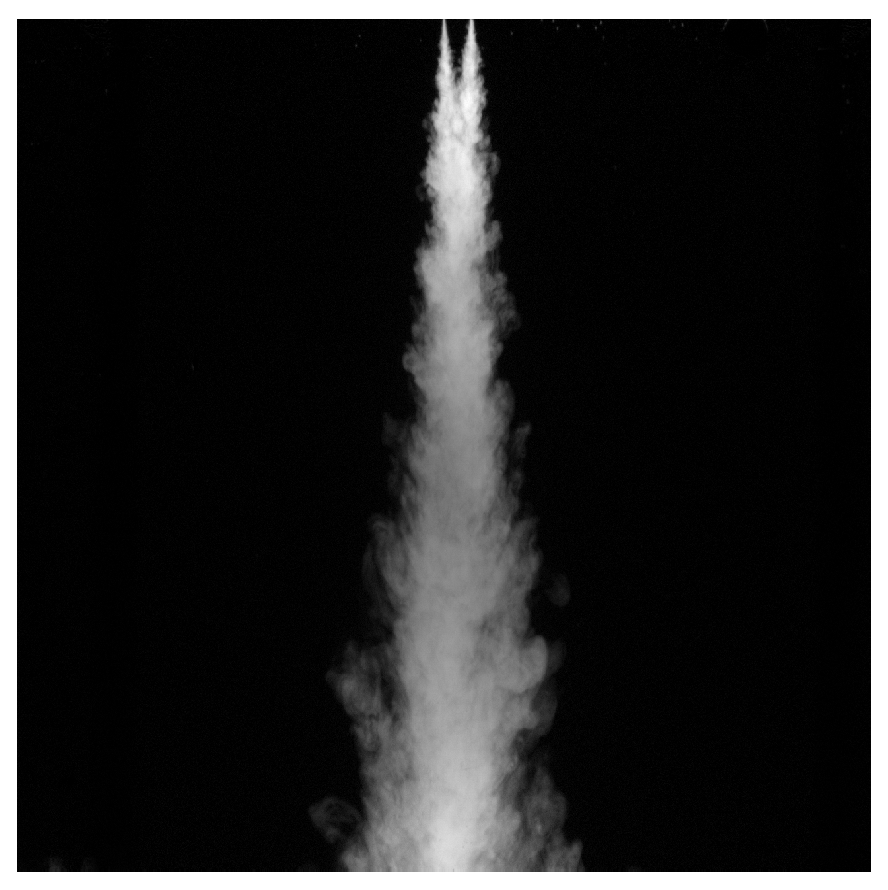
\includegraphics[trim = {0cm, 0cm, 0cm, 0cm}, clip, width = 0.45\textwidth, height = 2.6in, angle = 180]{frame650cleaned.eps}
		\hspace{1em}
		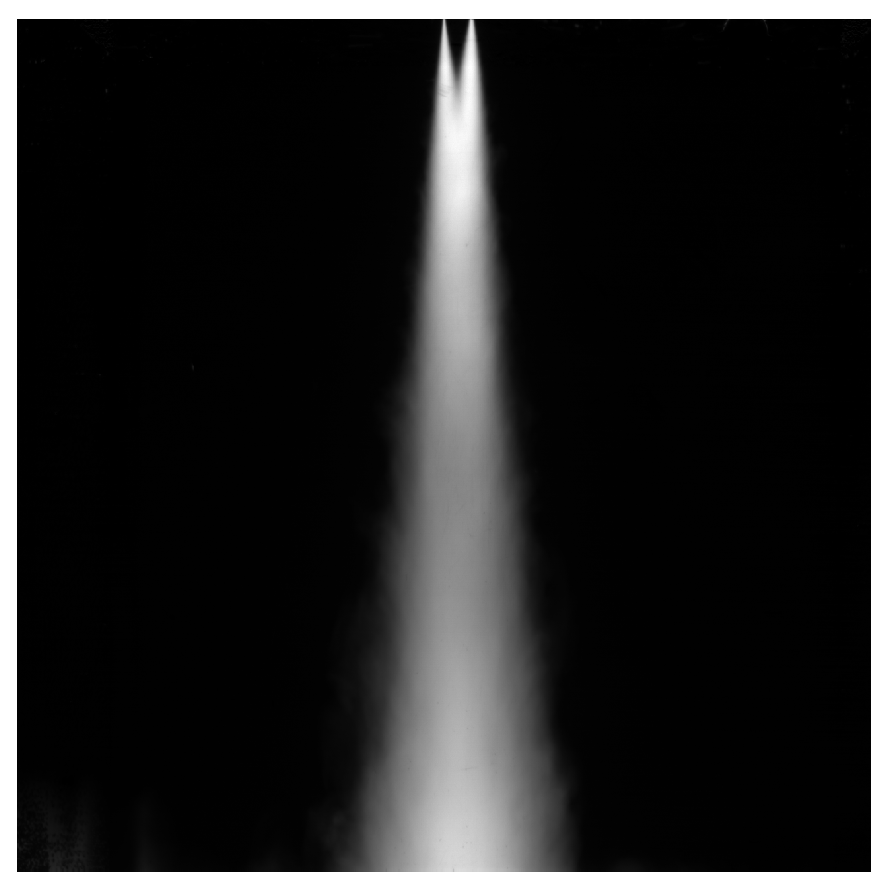
\includegraphics[trim = {0cm, 0cm, 0cm, 0cm}, clip, width = 0.45\textwidth, height = 2.6in, angle = 180]{twoPlumeAveraged.eps}
		\caption{Schematic of the dye attenuation technique. The background (top left) is subtracted from each from of footage (top right) to give a so-called ``subtracted image'' (bottom left). Time-averaging all subtracted images gives a single time-averaged image from the experiment (bottom right) }
		\label{fig:dyeAttenuation}
	\end{figure}
	
	
	
	 \begin{figure}
		\centering
			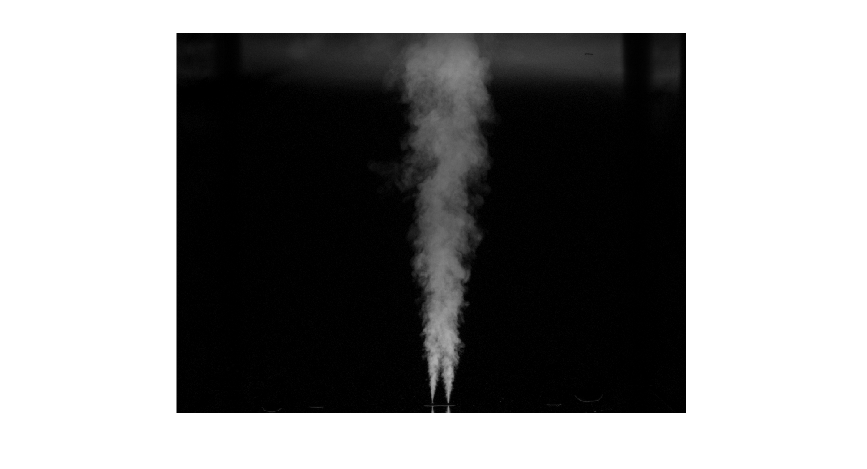
\includegraphics[trim = {5cm 0 5cm 2cm},clip,width =0.3\textwidth, height = 10cm]{twoNozzleInstantaneousExample.eps}
			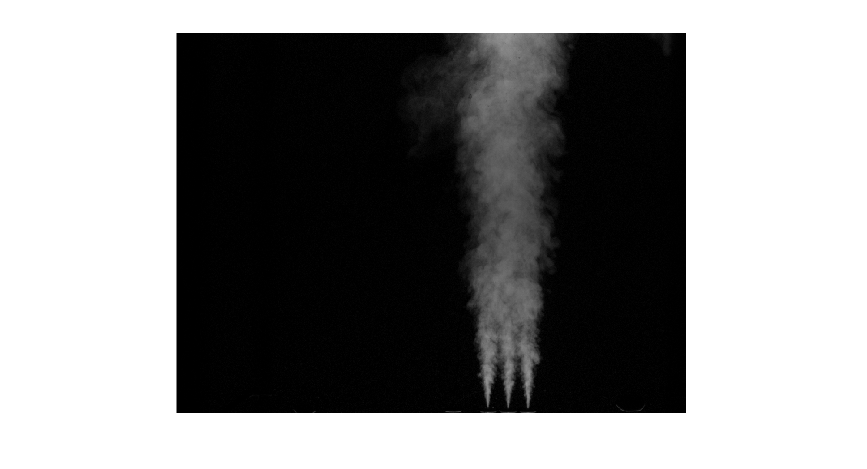
\includegraphics[trim = {6.5cm 0cm 4.5cm 2cm},clip,width = 0.3\textwidth,height = 10cm]{threeNozzleInstantaneousExample.eps}
			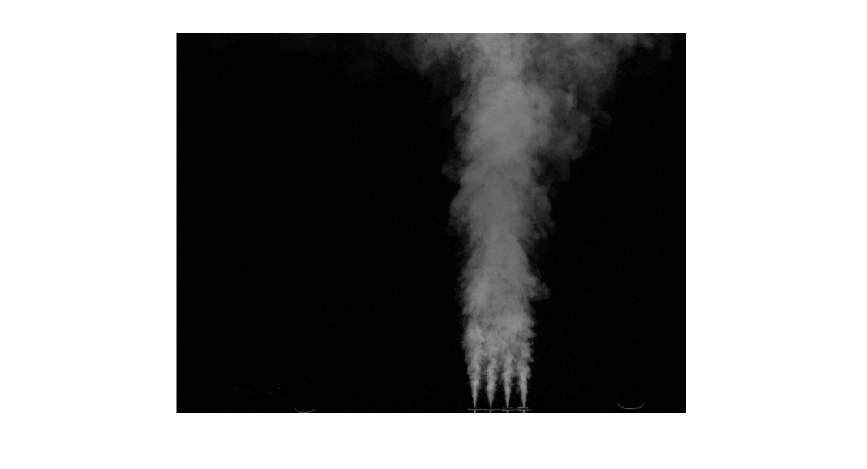
\includegraphics[trim = {6.5cm 0 4.5cm 2cm},clip,width = 0.3\textwidth,height = 10cm]{fourNozzleInstantaneousExample.eps}
		\vspace{-4em}
		\caption{ An instantaneous snapshot of the behaviour of two, three and four co-linear plumes 21.3 seconds after filming started. The plumes are configured such that each plume is separated from the adjacent plumes by $\chi_0 = $ 25\,mm.}
		\label{fig:instant snapshots}
	\end{figure}

    \begin{figure}
		\centering
			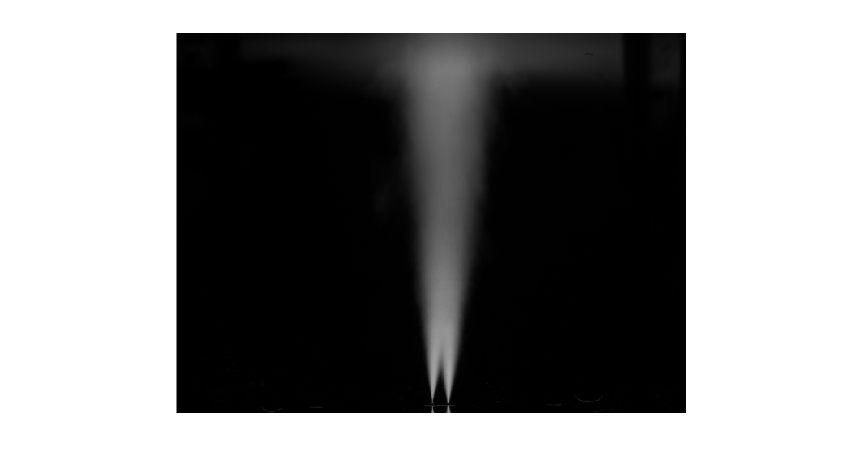
\includegraphics[trim = {5cm 0 5cm 2cm},clip,width = 0.3\textwidth, height = 10cm]{twoPlumeAverage.eps}
			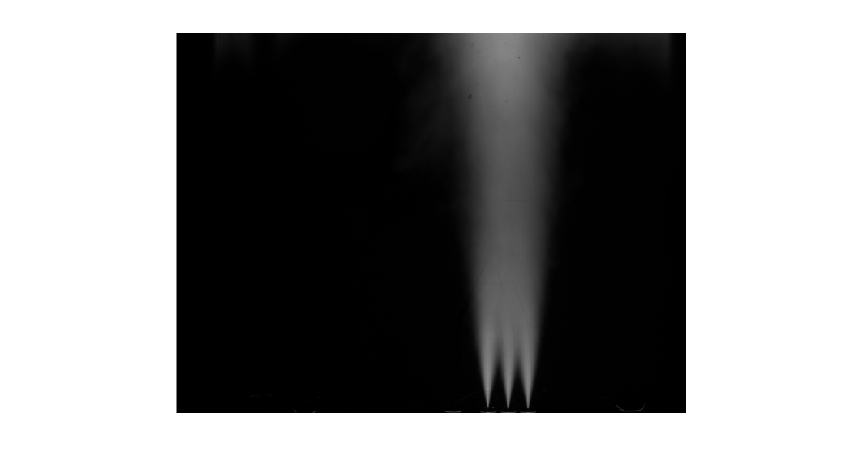
\includegraphics[trim = {6.5cm 0cm 4.5cm 2cm},clip,width = 0.3\textwidth,height = 10cm]{threePlumeAverage.eps}
			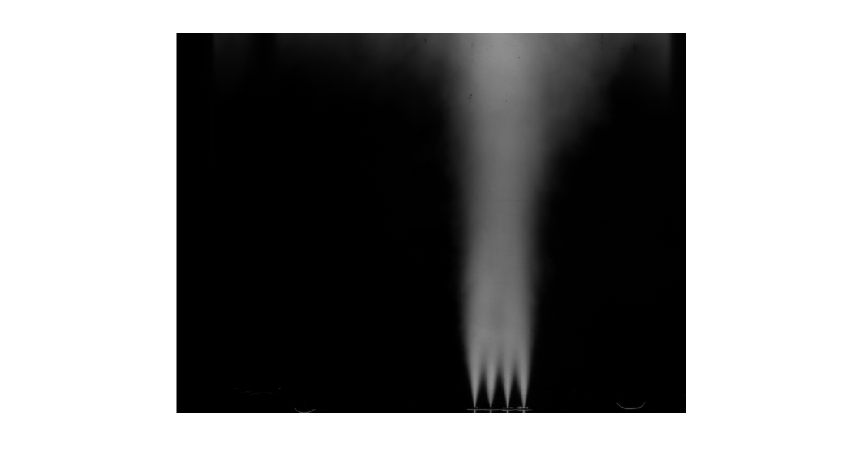
\includegraphics[trim = {6.5cm 0 4.5cm 2cm},clip,width = 0.3\textwidth,height = 10cm]{fourPlumeAverage.eps}
			\vspace{-4em}
		\caption{ Time-averaged behaviour of two, three and four co-linear plumes. The plumes are configured such that each plume is separated from the adjacent plumes by $\chi_0 = $25\,mm, and the data is formed from the frames of the 45 second video.}
		\label{fig:averaged images}
	\end{figure}
	\noindent The merging height may be determined using the time-averaged image. Recall, from SECREF, that the buoyancy profile of a plume is well approximated by a Gaussian, centred at the midline of the plume. Furthermore, it was shown, by CITE, that the buoyancy profile of a line of plumes may be approximated by a superposition of these Gaussians. Using this, we outline finding the merging height of two plumes, and note that it can be extended to an arbitrary line by adding more Gaussians, as shown in \eqref{eqn: n plume experimental buoyancy}.
	
	\par For each row of pixels of the time-averaged two-plume image, we fit a function of the form 
	\begin{equation}
		G = \dfrac{a_1}{a_2\sqrt{2\pi}}\exp\left(-\dfrac{(x-a_3)^2}{2a_2^2}\right) + \dfrac{a_4}{a_5\sqrt{2\pi}}\exp\left(-\dfrac{(x-a_6)^2}{2a_5^2}\right)\label{eqn:two plume experimental gaussian} 
	\end{equation}
	where $a_3$ and $a_6$ are the positions of maximum buoyancy, i.e. the centre of each plume. 
	For $n$ plumes, $G$ would take the form
	\begin{equation}
		G = \sum_{k = 1}^n \frac{a_{3k-2}}{a_{3k-1} \sqrt{2\pi}} \exp\left(-\frac{(x - a_{3k})^2}{2a_{3k-1}^2}\right). \label{eqn: n plume experimental buoyancy}
	\end{equation}

	\subsection{Results}
	By fitting \eqref{eqn:two plume experimental gaussian} to each row of pixels, we find the two peaked Gaussian that best fits the experimental data. This is repeated for each row of pixels until \eqref{eqn:two plume experimental gaussian} has a single maximum. This gives the vertical pixel at which the plumes have merged. This can then be converted to a real-world distance using the ``edit coordinates'' function in Digiflow. This converts pixel measurements to real-world measurements, based on known distances, using a least squares mapping. The real-world distance is the merging height of the system. \\
	
	\begin{figure}
			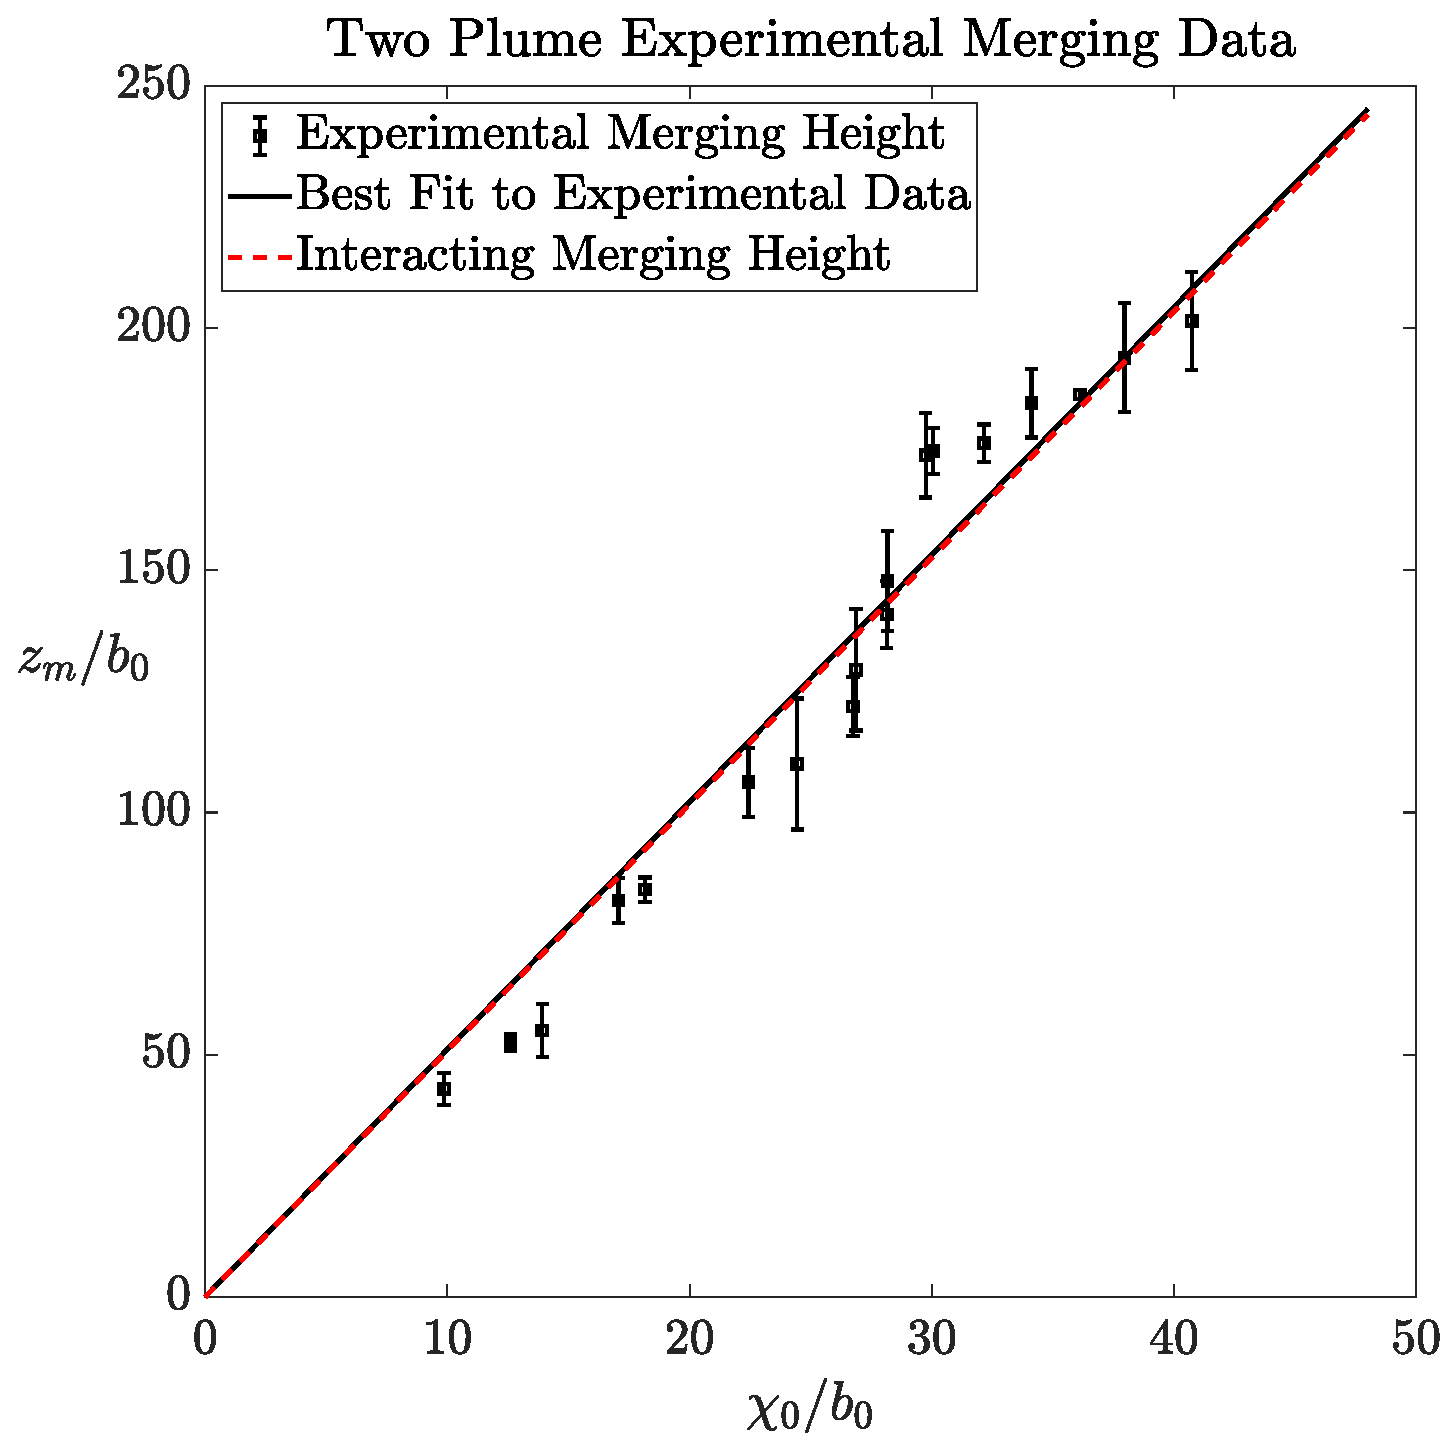
\includegraphics[width=0.45\textwidth]{twoPlumeDataWithErrorBars.eps}\hfill
			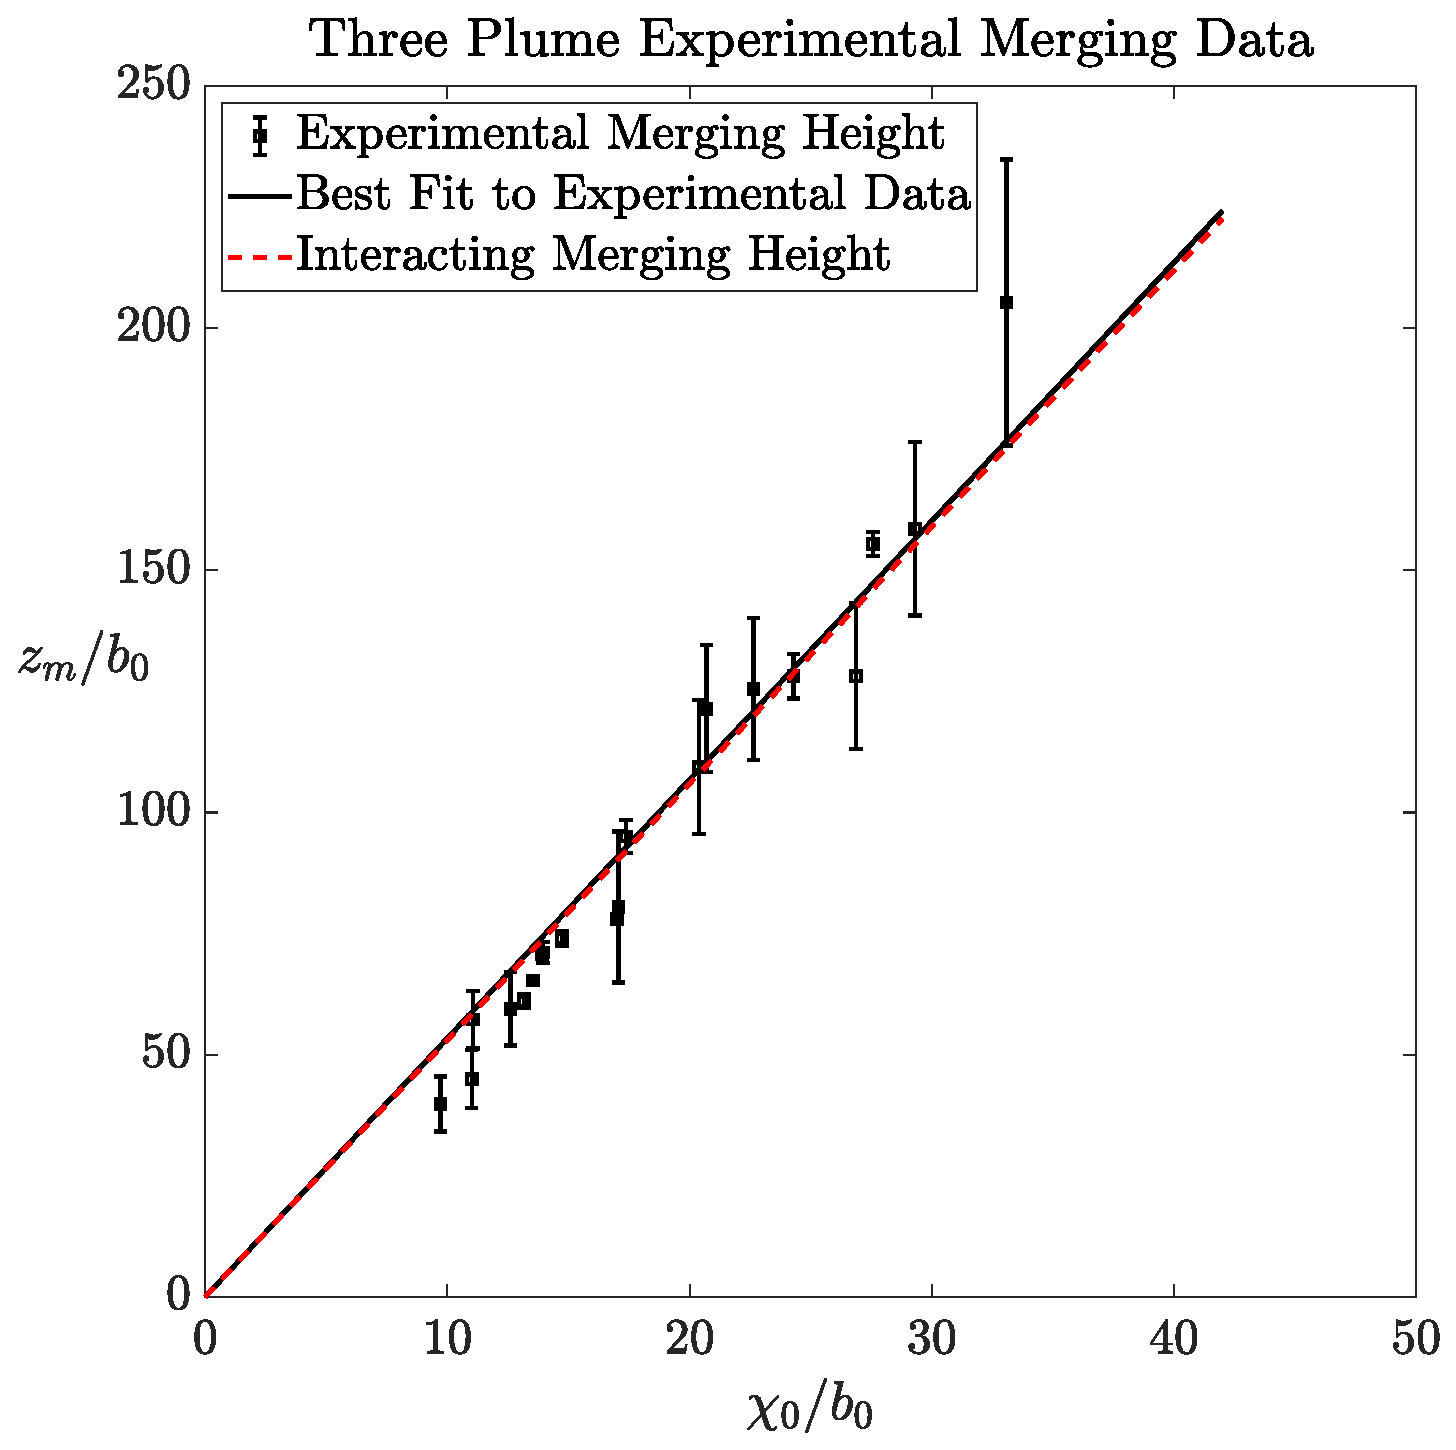
\includegraphics[width=0.45\textwidth]{threePlumeDataWithErrorBars.eps}
		
			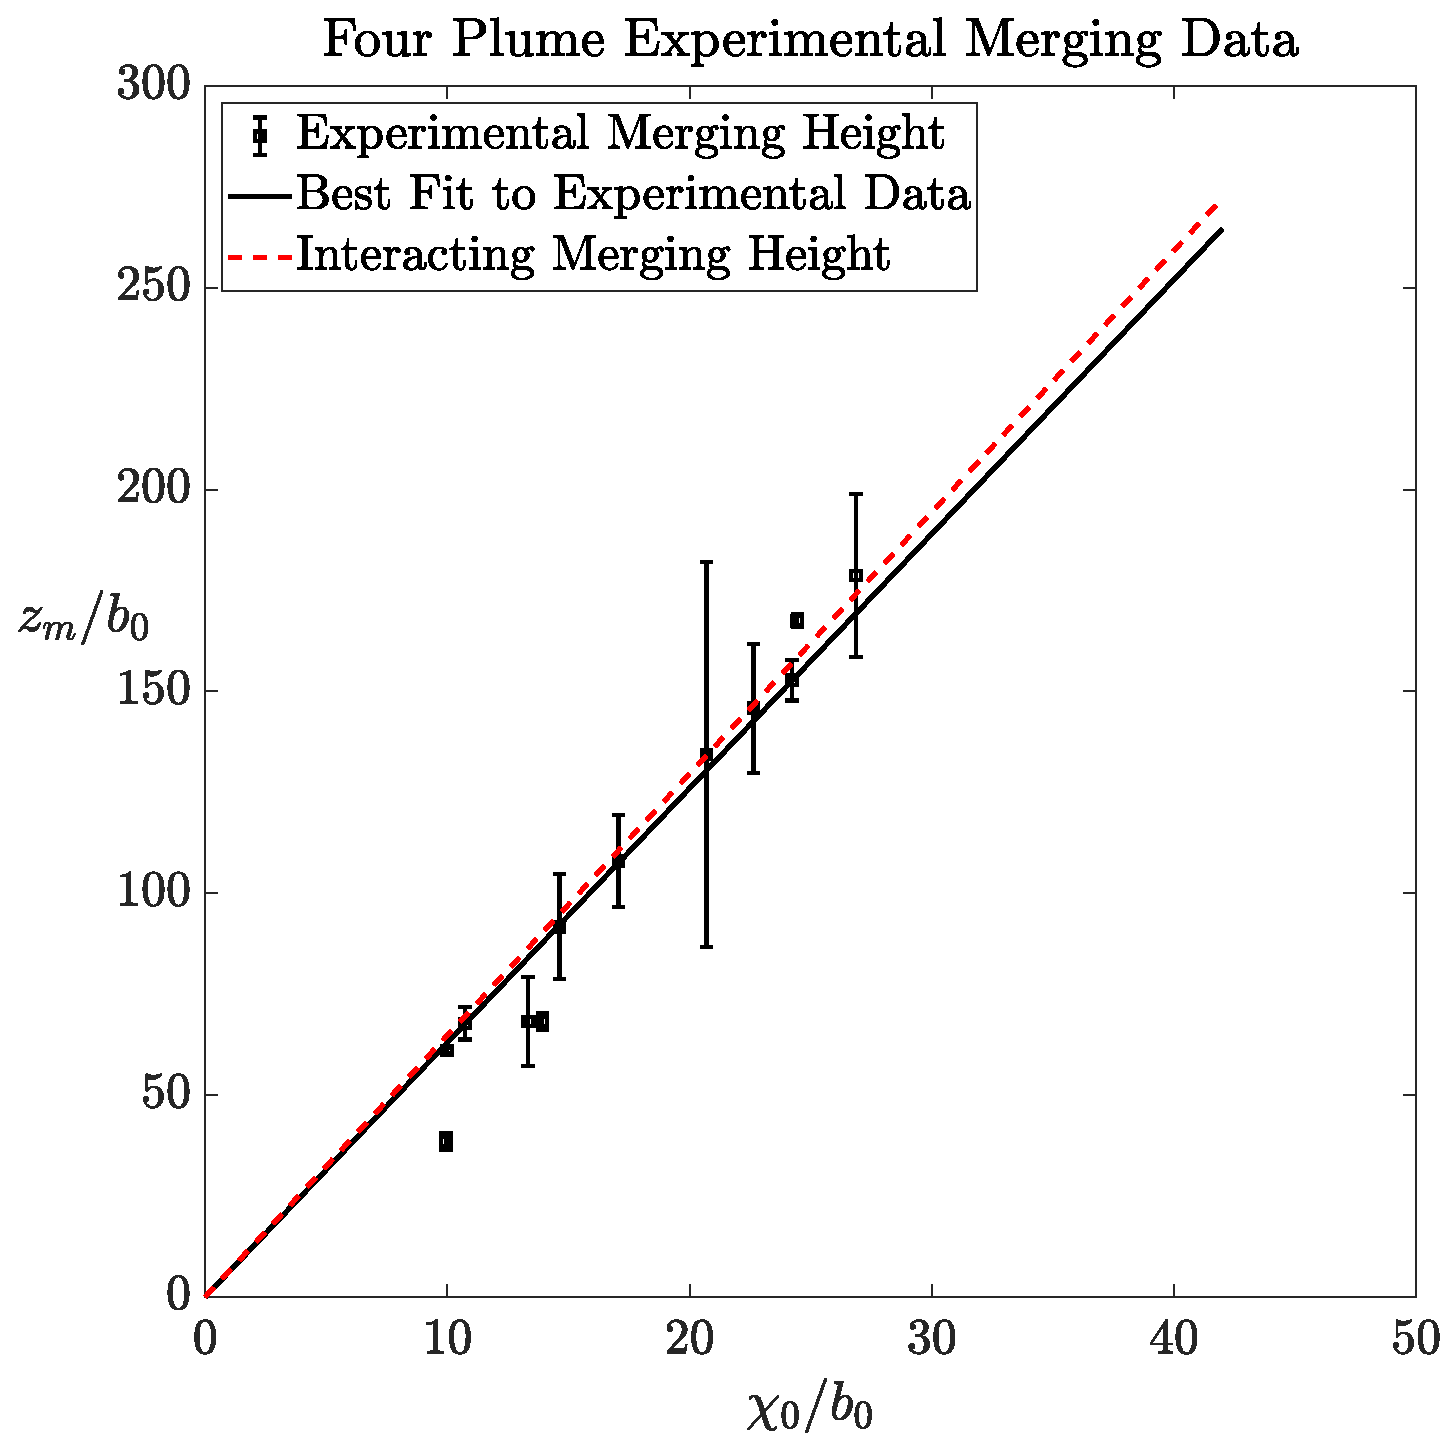
\includegraphics[width=0.45\textwidth]{fourPlumeDataWithErrorBars.eps}\hfill
			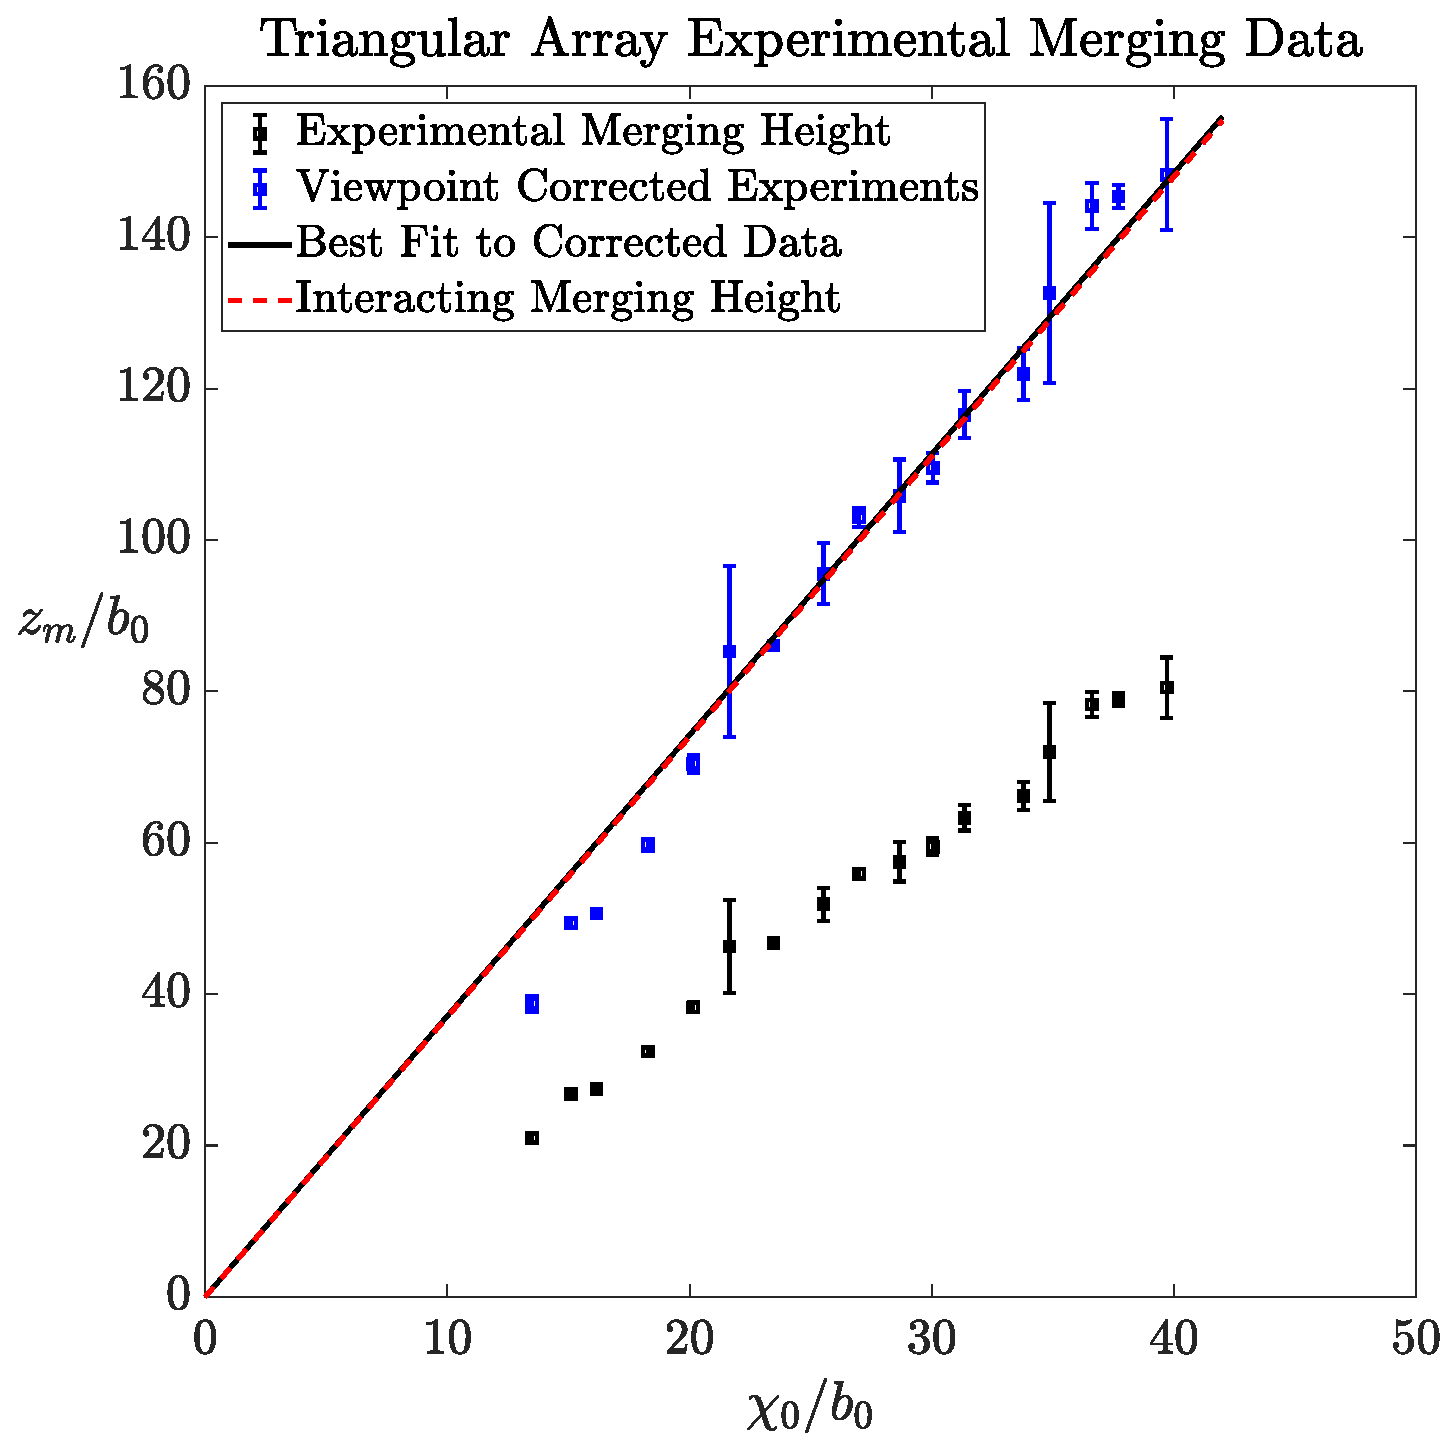
\includegraphics[width=0.45\textwidth]{triangularDataWithViewCorrectionAndErrorBars.eps}
		
			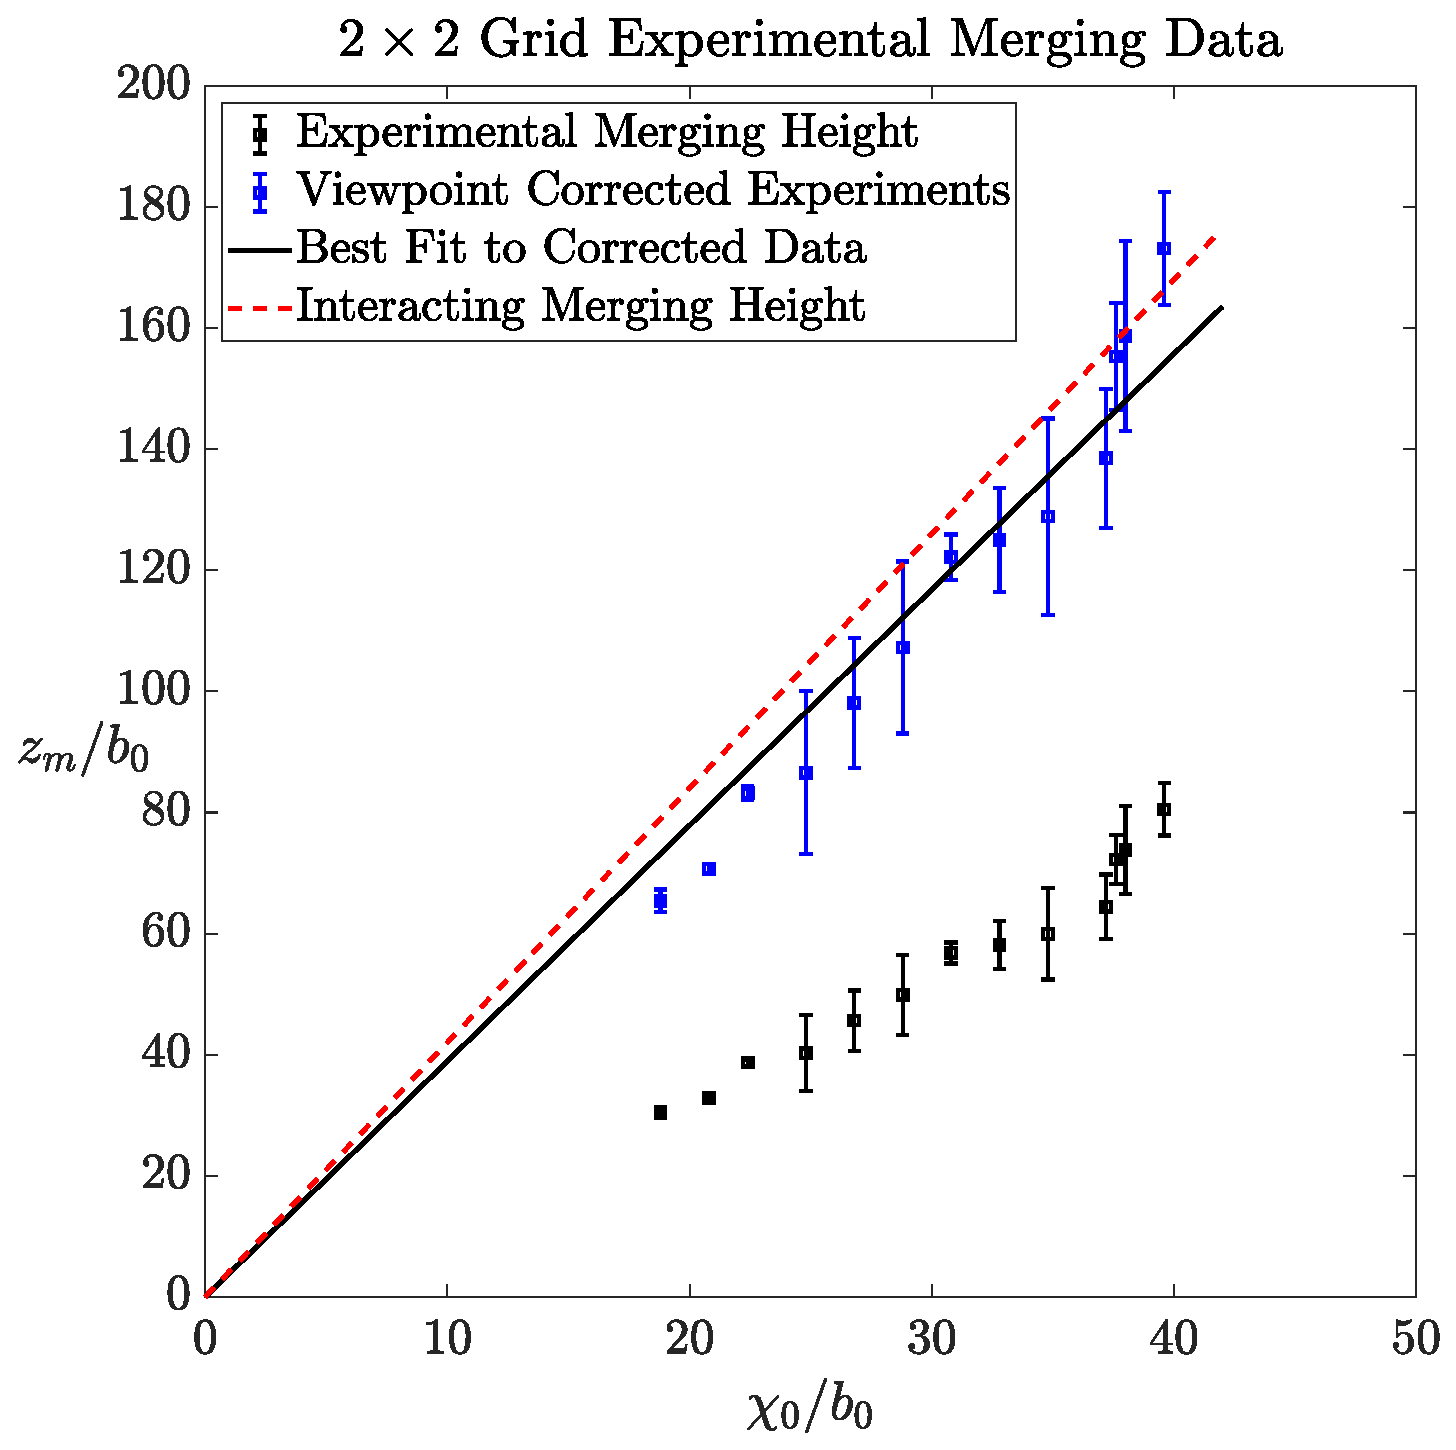
\includegraphics[width=0.45\textwidth]{gridDataWithViewCorrectionAndErrorBars.eps}\hfill
			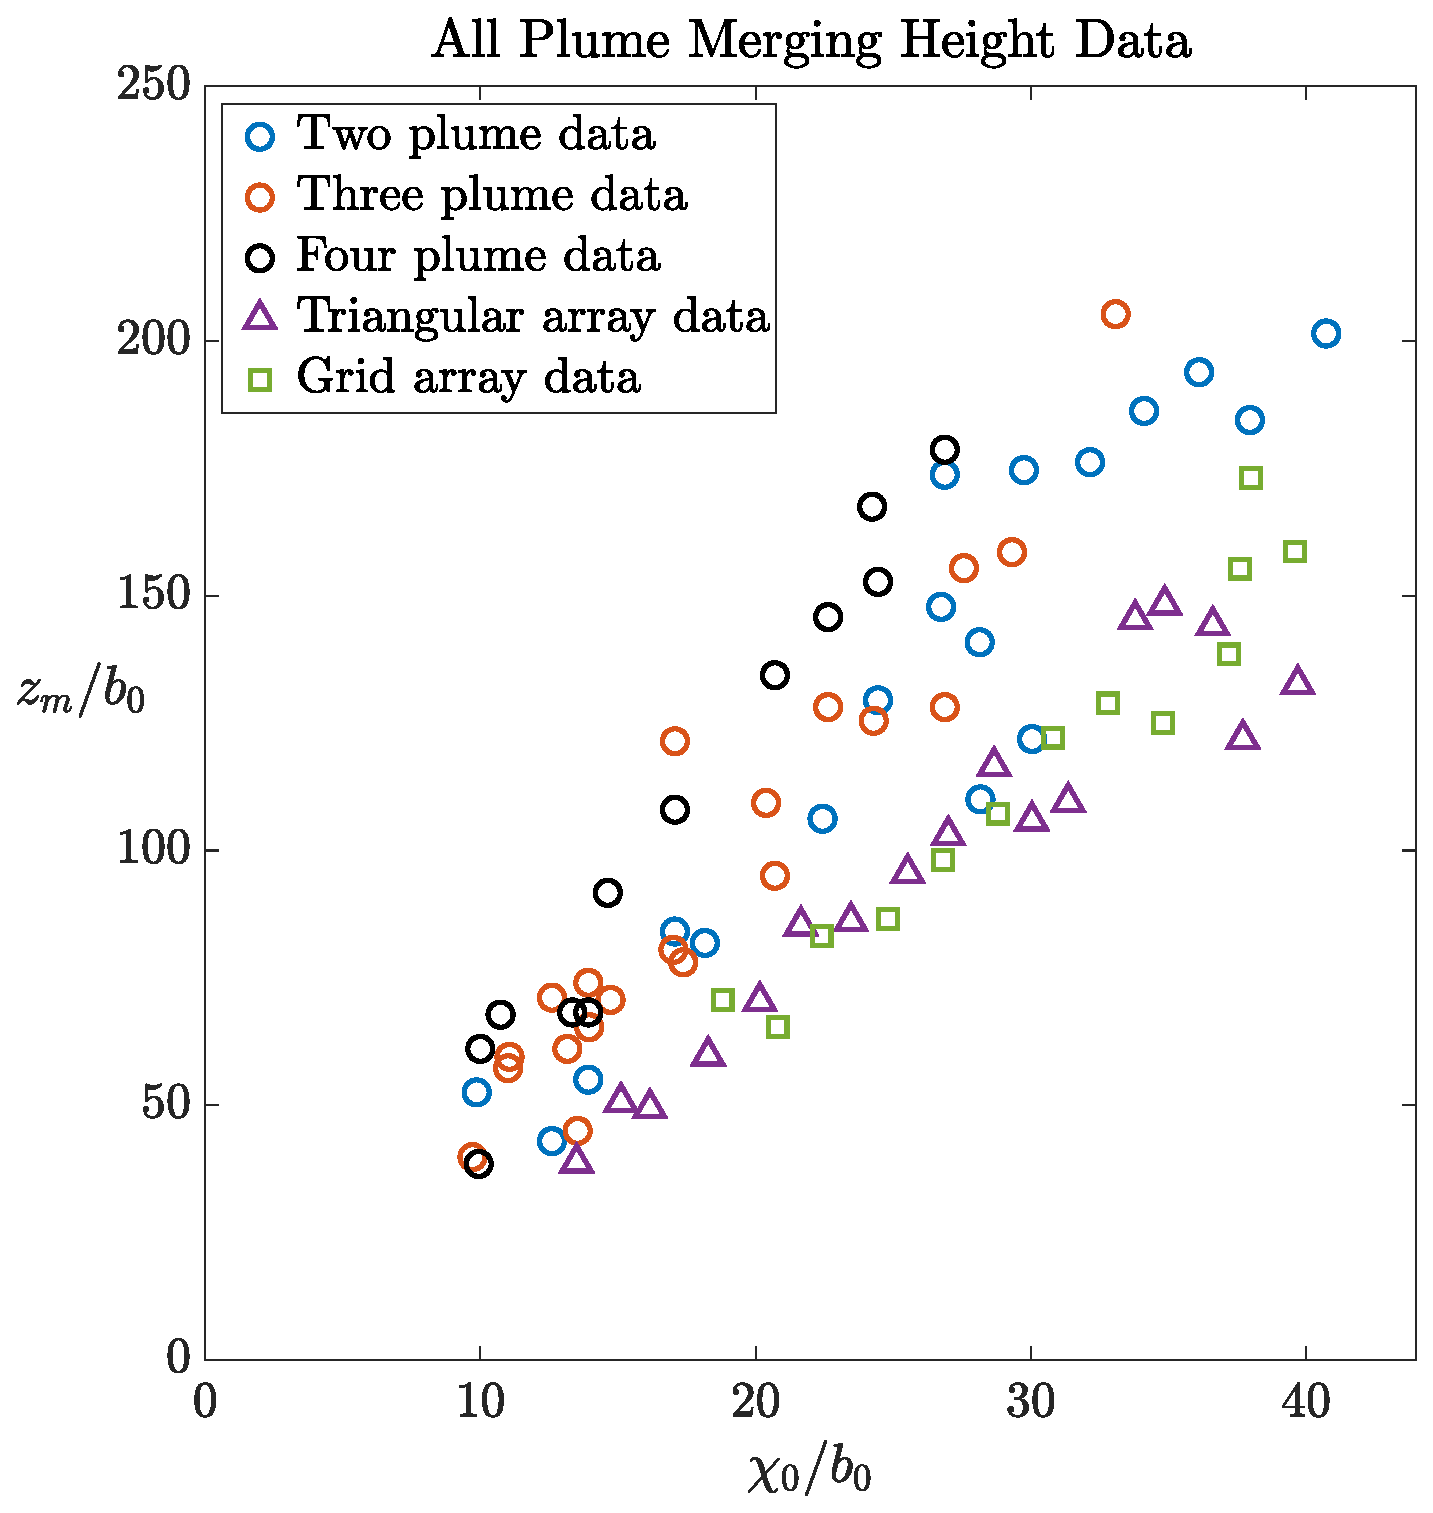
\includegraphics[width = 2.375in, height = 2.375in]{allDataCorrected.eps}
			\caption{.}
			\label{fig:experimental data}
	\end{figure}
	\noindent Following the procedure outlined in $\S$\ref{subsec:Data processing}, the experimental merging heights of each plume configuration was determined. By fitting a line of the form $z_{\text{me}} = \lambda_{\text{me}} \chi_0$ to the merging heights, we found the non-dimensional merging height for each configuration. The values for each configuration are given in table \ref{table:non-dimensional experimental merging heights with correction}. The merging heights for each configuration, as a function of separation, are plotted in figure \ref{fig:experimental data}.
	
	\subsubsection{Comparison to Models}
	Note that the imagery collected for the triangular and $2 \times 2$ grid array of plumes was only visualised by one camera, meaning it appeared as three or four co-linear plumes respectively. This led to an experimental merging height significantly lower than expected by the models in SECREF and SECREF. To correct for this, we simulated the array models for each experiment, and obtained the ``true'' merging height (the merging height of the array) and the ``observed'' merging height (the merging height obtained from the viewpoint in my experiments). A linear mapping was found between the observed and true merging heights for these arrays. By applying this mapping to my experimental data for the arrays of plumes, the visualisation error in these experiments was corrected. The experimental data, including the corrected data is shown in FIGREF. We see that by using the above correction, the experimental data is now in good agreement with the modelling outlined in SECREF, as shown in TABREF.
	
	\begin{table}
		\centering
		\begin{tabular}{lccc}
			Configuration & $\lambda_{\text{me}}$ & $\lambda_{m}^I$\\ [-5pt] \hline
			Line of two & 5.09 $\pm$ 5.57\% & 5.08\\
			Line of three & 5.32 $\pm$ 8.03\% & 5.30\\
			Line of four & 6.30 $\pm$ 9.86\% & 6.48\\
			Equilateral triangle & 3.69 $\pm$ 3.25\% & 3.70\\
			2 $\times$ 2 square grid & 3.89 $\pm$ 7.45\% & 4.20\\
		\end{tabular}
		\caption{ Non-dimensional merging heights of all experimental configurations and corresponding model merging heights with the corrected array data.}
		\label{table:non-dimensional experimental merging heights with correction}
	\end{table}
	\section{Conclusion}
This chapter has extended the work of SECREF, which sought to find the height at which a line of plumes would behave as a single, larger plume if interaction between plumes was ignored. An interacting model was devised, based on the assumption that the strength of plume interaction is inversely proportional to the distance between the plumes. For two plumes, this model collapses to the interacting model of Kaye \& Linden CITE. \\

\noindent This model was further generalised to an arbitrary, finite number of interacting co-linear plumes by considering the entrainment experienced by a plume due to its neighbours. Doing so led to the model given in SECREF. This model was extended to two arrays of interacting plumes - an equilateral triangle and a $2 \times 2$ grid. \\

\noindent The interacting models from SECREF were then compared to data collected from experiments for five configurations. The method of data collection and extraction of the merging height from the experimental data was outlined. The models were compared to the experimental data in FIGREF. We saw that these interacting models were in good agreement with the experimental data. 
\bibliographystyle{jfm}
\bibliography{stillwater.bib}
\end{document}
